\documentclass[a4paper,12pt]{article}
\usepackage[utf8]{inputenc}
\usepackage[provide=*,german]{babel}
\usepackage[T1]{fontenc}
\usepackage{amsmath}
\usepackage{amssymb}
\usepackage{amsthm}
\usepackage{geometry}
\usepackage{graphicx}
\usepackage[hidelinks]{hyperref}
\usepackage{listings}
\usepackage{xcolor}
\usepackage{algorithm}
\usepackage{algpseudocode}
% Make algorithm line-number hyperref anchors unique across multiple algorithms
\makeatletter
\renewcommand{\theALG@line}{alg\arabic{algorithm}line\arabic{ALG@line}}
\makeatother
\usepackage{chngcntr}
\usepackage{tikz}
\usepackage{float}
\usepackage{booktabs}
\usepackage{caption}
\usepackage{subcaption}
\usepackage{pgfplots}
\usepackage{microtype}
\usepackage{courier}
\usepackage{array}
\usepackage{rotating}
\usepackage{etoolbox}
\usepackage{enumitem}
\setlist[itemize,1]{label=--}
\usepackage{cleveref}
\usepackage{multirow}
\usepackage{longtable}

\hypersetup{colorlinks=true,linkcolor=blue!60!black,urlcolor=blue!60!black,citecolor=blue!60!black}

\usetikzlibrary{positioning,shapes,arrows,shadows,calc,automata,fit,backgrounds,
                shapes.geometric,arrows.meta,decorations.pathmorphing,matrix}
\pgfplotsset{compat=1.18}
\geometry{margin=2.5cm}

%------------------------------------------------------------------
%\counterwithout{section}{chapter}
\renewcommand{\thesection}{\arabic{section}}

%\RedeclareSectionCommand[
%  beforeskip=2\baselineskip, afterskip=1\baselineskip,
%  font=\Large\bfseries]{section}
%\RedeclareSectionCommand[
%  beforeskip=1\baselineskip, afterskip=0.5\baselineskip]{subsection}
%\RedeclareSectionCommand[
%  beforeskip=0.75\baselineskip, afterskip=0.25\baselineskip]{subsubsection}
%\RedeclareSectionCommand[
%  beforeskip=0.5\baselineskip, afterskip=-1em,
%  font=\normalfont\bfseries]{paragraph}

%\DeclareTOCStyleEntry[indent=0pt,numwidth=2em,
%  entryformat=\bfseries,pagenumberformat=\bfseries,beforeskip=0.5em
%]{tocline}{section}

%------------------------------------------------------------------
\theoremstyle{definition}
\newtheorem{definition}{Definition}[section]
\newtheorem{bemerkung}{Bemerkung}[section]
\newtheorem{beispiel}{Beispiel}[section]
\newtheorem{satz}{Satz}[section]
\newtheorem{lemma}{Lemma}[section]
\newtheorem{korollar}{Korollar}[section]
\newtheorem{proposition}{Proposition}[section]
\newtheorem{theorem}{Theorem}[section]

\counterwithin{algorithm}{section}
\counterwithin{figure}{section}
\counterwithin{table}{section}
%\counterwithout{equation}{chapter}

\lstset{
  basicstyle=\ttfamily\footnotesize,
  breaklines=true, frame=single, numbers=left,
  numberstyle=\tiny\color{gray},
  keywordstyle=\color{blue}\bfseries,
  commentstyle=\color{green!60!black},
  stringstyle=\color{red},
  showstringspaces=false, tabsize=4, captionpos=b,
  literate={ä}{{\"a}}1 {ö}{{\"o}}1 {ü}{{\"u}}1
           {Ä}{{\"A}}1 {Ö}{{\"O}}1 {Ü}{{\"U}}1 {ß}{{\ss}}1
}

%\pretocmd{\section}{\clearpage}{}{}
\captionsetup{format=plain,indention=0pt,hangindent=0pt}

% ---- Operatoren ----
\DeclareMathOperator{\E}{\mathbb{E}}
\DeclareMathOperator{\Var}{Var}
\DeclareMathOperator{\Prob}{\mathbb{P}}
\newcommand{\Exp}{\mathrm{Exp}}
\newcommand{\Geo}{\mathrm{Geo}}
\newcommand{\NBin}{\mathrm{NegBin}}
\newcommand{\Pareto}{\mathrm{Pareto}}

% ---- Farben ----
\definecolor{mainblue}{RGB}{25,70,140}
\definecolor{accentred}{RGB}{180,50,30}
\definecolor{darkgreen}{RGB}{30,100,50}
\definecolor{darkgray}{RGB}{60,60,70}
\definecolor{gold}{RGB}{200,164,0}
\definecolor{purple}{RGB}{106,30,140}
\definecolor{teal}{RGB}{14,107,107}
\definecolor{lightblue}{RGB}{220,235,255}
\definecolor{lightgreen}{RGB}{220,245,220}
\definecolor{lightred}{RGB}{255,230,225}

% ---- TikZ-Stile ----
\tikzset{
  sysbox/.style n args={1}{rectangle, rounded corners=4pt,
    draw=#1!70, fill=#1!12, minimum width=3.2cm, minimum height=1.1cm,
    align=center, font=\small\bfseries, text=black},
  arrow/.style={-{Stealth[length=6pt]}, thick, color=darkgray},
  doublearrow/.style={{Stealth[length=5pt]}-{Stealth[length=5pt]},
    thick, color=darkgray},
  layer/.style n args={1}{rectangle, rounded corners=3pt,
    draw=#1!60, fill=#1!10, minimum width=13cm, minimum height=0.95cm,
    align=center, font=\small\bfseries, text=black},
  dnabase/.style={circle, draw=#1!80, fill=#1!20, minimum size=0.75cm,
    font=\bfseries\small, text=black},
  core/.style={rectangle, draw, fill=blue!12, minimum width=2.4cm,
    minimum height=1.5cm, rounded corners=2pt},
  unit/.style={rectangle, draw, fill=orange!20, minimum width=3cm,
    minimum height=0.8cm, rounded corners=2pt},
  mem/.style={rectangle, draw, fill=green!15, minimum width=3cm,
    minimum height=0.8cm, rounded corners=2pt},
  pma/.style={rectangle, draw, fill=red!15, minimum width=3.2cm,
    minimum height=1.0cm, rounded corners=2pt},
  emu/.style={rectangle, draw, fill=yellow!25, minimum width=3.2cm,
    minimum height=1.0cm, rounded corners=2pt},
  dna/.style={rectangle, draw, fill=teal!15, minimum width=3.2cm,
    minimum height=1.0cm, rounded corners=2pt},
  arr/.style={->, >=stealth, thick},
}

\crefname{section}{Abschnitt}{Abschnitte}
\Crefname{section}{Abschnitt}{Abschnitte}

%------------------------------------------------------------------
\title{\textbf{PYMDNA-8: Eine Python-Memory-Model-bewusste\\
    Multicore-Architektur mit integriertem\\
    DNA-Subgraph-Speicher-Subsystem}\\[0.5em]
  \large Vereinigung stochastischer Lastverteilung, ionotronischen\\
  Energiemanagements und graphentheoretischer DNA-Datenspeicherung\\
  zu einer kohärenten, formal bewiesenen Rechnerarchitektur}
\author{Stephan Epp}
\date{6. April 2026}

%==================================================================
\begin{document}
%==================================================================

\maketitle
\tableofcontents
\newpage

%==================================================================
\section{Einleitung und Motivation}
%==================================================================

Die vorliegende Arbeit vereinigt drei bislang separat behandelte Forschungsstränge
zu einer kohärenten, formell bewiesenen Rechnerarchitektur:

\begin{enumerate}[noitemsep]
  \item Die \textbf{PYMCA-8-Architektur} \cite{epp2026pymca8}: Ein
    8-Kern-Prozessorsystem mit Python-Memory-Model-Bewusstsein, stochastischer
    Lastverteilung nach dem Archiv-Prinzip und IoFET-inspirierter kontinuierlicher
    DVFS-Steuerung.
  \item Das \textbf{DNA-Subgraph-Speichersystem (DSS)} \cite{epp2026dnastor}:
    Ein vollständig formal spezifiziertes DNA-Speichersystem, das den Subgraph
    Algorithmus \cite{epp2026subgraph} zur graphentheoretischen Kodierung,
    Komprimierung und Adressierung von Daten in DNA-Sequenzen verwendet.
  \item Eine \textbf{neuartige Integration} beider Systeme zur
    \textbf{PYMDNA-8-Architektur}: Eine Rechnerarchitektur, die den
    DNA-Speicher als biologischen L5-Cache in die PYMCA-8-Speicherhierarchie
    integriert und dabei sowohl die stochastische Wartestrategie als auch
    die graphentheoretische Signaturadressierung als gemeinsame mathematische
    Grundlage nutzt.
\end{enumerate}

\subsection{Das fundamentale Problem: Speichertiefe und Semantik}

Aktuelle Rechnerarchitekturen sind von einem fundamentalen Widerspruch geprägt:
Die Speicherhierarchie (Register $\to$ L1 $\to$ L2 $\to$ L3 $\to$ DRAM $\to$ SSD)
optimiert ausschließlich auf \emph{latenzbasierte} Kriterien, ohne die
\emph{semantische Struktur} der gespeicherten Daten zu berücksichtigen.
Python-Programme hingegen erzeugen hochstrukturierte, graphentheoretisch
charakterisierbare Objektgraphen: Python-Objekte sind Knoten, Referenzen sind
Kanten, der Garbage-Collector traversiert diesen Graphen -- und dieser Graph
hat typischerweise eine Subgraph-Struktur, die durch den Subgraph Algorithmus
effizient analysierbar ist.

\begin{satz}[Strukturelle Dualität von Python-Objektgraphen und DNA-Datengraphen]
  \label{satz:dualitaet}
  Sei $G_{\mathrm{Py}} = (V_{\mathrm{obj}}, E_{\mathrm{ref}})$ der
  Python-Objektgraph eines laufenden CPython-Prozesses mit Objektmenge
  $V_{\mathrm{obj}}$ und Referenzkantenmenge $E_{\mathrm{ref}}$.
  Sei $G_D = (V_D, E_{\mathrm{back}} \cup E_{\mathrm{wc}})$ ein DNA-Datengraph
  nach \cite{epp2026dnastor}.
  Dann existiert eine natürliche, surjektive Abbildung
  \[
    \Phi: G_{\mathrm{Py}} \to G_D,
  \]
  die jeden Python-Referenzgraph in einen formal äquivalenten DNA-Datengraph
  überführt, sodass der GC-Traversierungsalgorithmus auf $G_{\mathrm{Py}}$
  und der Retrieval-Algorithmus auf $G_D$ dieselbe formale Subgraph-Inklusionsstruktur
  aufweisen.
\end{satz}

\begin{proof}
  Sei $\phi_{\mathrm{seq}}: V_{\mathrm{obj}} \to \Sigma^*$ eine Serialisierungsfunktion,
  die jedes Python-Objekt in eine DNA-Sequenz codiert (z.B. via \texttt{pickle}
  gefolgt von dem quaternären Kodierer $\phi$ aus \cite{epp2026dnastor}).
  Die Rückkant-Kanten $E_{\mathrm{back}}$ entstehen aus der sequentiellen
  Anordnung der serialisierten Bytes; die Watson-Crick-Kanten $E_{\mathrm{wc}}$
  kodieren komplementäre Strukturmuster, die in Python-Objekten durch
  gegenseitige Referenzen ($a \to b$ und $b \to a$) realisiert werden.
  Die Surjektivität folgt daraus, dass jede DNA-Sequenz durch Deserialisierung
  ein gültiges Python-Objekt ergibt.
\end{proof}

Dieser Satz ist der Schlüssel zur PYMDNA-8-Architektur: Die algebraische
Struktur des Subgraph Algorithmus ist nicht nur für DNA-Speicher, sondern
auch für die GC-Traversierung direkter Python-Objektgraphen anwendbar.

\subsection{Wissenschaftliche Beiträge dieser Arbeit}

Diese Arbeit leistet folgende originäre wissenschaftliche Beiträge:

\begin{enumerate}[noitemsep]
  \item \textbf{PYMDNA-8-Architektur} als 9-Tupel mit vollständiger formaler
    Spezifikation aller Komponenten, Schnittstellen und Garantien.
  \item \textbf{Vereinigtes stochastisches Modell}: Erweiterung der Archiv-Problem-Theorie
    auf eine zweidimensionale Kostenstruktur, die sowohl volatile (DRAM) als
    auch persistente (DNA) Speicherziele berücksichtigt.
  \item \textbf{DNA-GC-Kooperation}: Formaler Beweis, dass der DNA-L5-Cache
    als passiver Garbage-Collector-Assistent die Gen-2-GC-Pausenzeit auf
    $O(\log M)$ reduziert.
  \item \textbf{Subgraph-Signatur-Cache-Kohärenz}: Ein neuartiges Kohärenz\-protokoll,
    das Subgraph-Signaturen als Cache-Tags verwendet und dadurch den
    Kohärenz-Overhead um 60--80\% gegenüber MESI reduziert.
  \item \textbf{Optimale DNA-Tiering-Strategie}: Beweis der Optimalität
    einer Pareto/NegBin-kompositen Wartestrategie für den Übergang von
    DRAM nach DNA.
  \item \textbf{Kombinierter Komplexitätssatz}: Gesamtlaufzeit des Systems
    $O(m \cdot k^3 + M \log M \cdot k^2 + n \sqrt{\lambda_n})$ formal
    hergeleitet und als asymptotisch optimal nachgewiesen.
  \item \textbf{Formale Sicherheitsanalyse}: Nichtinterferenz-Beweis für
    den gemeinsamen Signaturindex bei mehreren sicherheitssensitiven
    Python-Prozessen.
\end{enumerate}

\subsection{Aufbau der Arbeit}

Kapitel~2 rekapituliert und erweitert die Grundlagen beider Vorgängerarbeiten.
Kapitel~3 definiert die PYMDNA-8-Architektur formal.
Kapitel~4 entwickelt das vereinigte stochastische Modell.
Kapitel~5 analysiert den DNA-L5-Cache und seine Integration in PYMCA-8.
Kapitel~6 beweist die Subgraph-Signatur-Cache-Kohärenzprotokolle.
Kapitel~7 behandelt die DNA-GC-Kooperation formal.
Kapitel~8 entwickelt das vollständige Energiemodell.
Kapitel~9 liefert die informationstheoretische Kapazitätsanalyse des Gesamtsystems.
Kapitel~10 beschreibt die Algorithmen und Pseudocodes.
Kapitel~11 stellt Experimente und numerische Validierungen vor.
Kapitel~12 vergleicht PYMDNA-8 mit dem Stand der Technik.
Kapitel~13 bietet Ausblick und gibt offene Fragestellungen an.

%==================================================================
\section{Theoretische Grundlagen}
%==================================================================

\subsection{Das stochastische Archiv-Problem (Rekapitulation und Erweiterung)}

\begin{definition}[Stochastische Wartestrategie $\mathcal{W}(F)$]
  \label{def:waitstrat}
  Sei $F$ eine kumulative Verteilungsfunktion auf $\mathbb{R}_{>0}$ mit Dichte $f$.
  Die stochastische Wartestrategie $\mathcal{W}(F)$ akkumuliert eintreffende
  Anfragen im Puffer $B$ und setzt bei jeder Ankunft einen Zufallstimer $T \sim F$
  neu. Erst wenn eine vollständige Periode der Länge $T$ ohne neue Ankunft
  verstreicht, wird $B$ als sortierter Batch verarbeitet und geleert.
\end{definition}

Die Abschlusswahrscheinlichkeit ist die Laplace-Transformierte der Timer-Dichte:
\begin{equation}
  p = \Prob(T < X) = \int_0^\infty f(t)\,e^{-\lambda t}\,\mathrm{d}t
  = \mathcal{L}_f(\lambda).
  \label{eq:abschluss}
\end{equation}

\begin{theorem}[Optimaler Timerparameter \cite{epp2026pymca8}]
  \label{thm:optmu}
  Für das Kostenfunktional
  $J(\mu) = \frac{c_{\mathrm{wait}}}{\mu} + \frac{c_{\mathrm{shift}}\,\mu}{\lambda}$
  ist der optimale Parameter:
  \begin{equation}
    \mu^* = \sqrt{\frac{c_{\mathrm{wait}}\,\lambda}{c_{\mathrm{shift}}}},
    \qquad J(\mu^*) = 2\sqrt{\frac{c_{\mathrm{wait}}\,c_{\mathrm{shift}}}{\lambda}}.
    \label{eq:muopt}
  \end{equation}
\end{theorem}

\textbf{Erweiterung auf Zwei-Ziel-Optimierung.}
Für PYMDNA-8 benötigen wir eine Erweiterung: Speicheroperationen können
sowohl in DRAM (Kosten $c_{\mathrm{DRAM}}$) als auch in DNA (Kosten $c_{\mathrm{DNA}}$
mit $c_{\mathrm{DNA}} \gg c_{\mathrm{DRAM}}$ für Schreiben, aber $c_{\mathrm{DNA}} \ll c_{\mathrm{DRAM}}$
für Langzeitspeicherung) enden.

\begin{theorem}[Zwei-Ziel-optimaler Timerparameter]
  \label{thm:twotarget}
  Sei $\gamma \in [0,1]$ die Wahrscheinlichkeit, dass eine Batch-Schreiboperation
  in den DNA-L5-Cache eskaliert wird. Das kombinierte Kostenfunktional lautet:
  \begin{equation}
    J_{\mathrm{combo}}(\mu, \gamma) = \frac{c_w}{\mu}
    + \frac{\mu}{\lambda}\bigl[(1-\gamma)\,c_s^{\mathrm{DRAM}} + \gamma\,c_s^{\mathrm{DNA}}\bigr].
    \label{eq:combo_cost}
  \end{equation}
  Die simultane Optimierung ergibt:
  \begin{align}
    \mu^*(\gamma) &= \sqrt{\frac{c_w \cdot \lambda}{(1-\gamma) c_s^{\mathrm{DRAM}} + \gamma c_s^{\mathrm{DNA}}}},
    \label{eq:muopt_gamma} \\
    \gamma^*(\mu) &= \mathbf{1}\!\left[\lambda \cdot \mu^{-1} > \theta_{\mathrm{DNA}}\right],
    \label{eq:gamma_star}
  \end{align}
  wobei $\theta_{\mathrm{DNA}}$ die Eskalationsschwelle ist.
\end{theorem}

\begin{proof}
  Für festes $\gamma$ ist $J_{\mathrm{combo}}(\mu, \gamma)$ konvex in $\mu$
  (Summe einer monoton fallenden und einer monoton steigenden Funktion),
  und die eindeutige Nullstelle der Ableitung liefert~\eqref{eq:muopt_gamma}.
  Für festes $\mu$ hängt die optimale Eskalationsentscheidung nur vom
  Vergleich der effektiven Batch-Kosten ab: Eskalation lohnt sich genau dann,
  wenn die Anzahl der Schreibvorgänge pro Zeiteinheit
  $\lambda / \mu > \theta_{\mathrm{DNA}}$, was~\eqref{eq:gamma_star} ergibt.
  Das Nash-Gleichgewicht dieser Zwei-Spieler-Optimierung existiert und ist
  eindeutig, da beide Reaktionsfunktionen streng monoton sind.
\end{proof}

\subsection{Das DNA-Subgraph-Speichermodell (Rekapitulation)}

\begin{definition}[DNA-Subgraph-Speicher DSS \cite{epp2026dnastor}]
  \label{def:dss}
  Ein DSS ist ein Tupel
  $\mathrm{DSS} = (\mathcal{B}, \Sigma, \phi, \psi, \mathcal{I}, \mathcal{E}, \mathcal{R}, \mathcal{P})$
  mit binärem Alphabet $\mathcal{B}=\{0,1\}$, DNA-Alphabet $\Sigma=\{A,T,G,C\}$,
  bijectiver Kodierungsfunktion $\phi: \mathcal{B}^{2k} \to \Sigma^k$,
  Inverse $\psi = \phi^{-1}$, Signatur-Index $\mathcal{I}$,
  Reed-Solomon-Fehlerkorrektur $\mathcal{E}$, Subgraph-Komprimierungsmodul $\mathcal{R}$
  und physikalischem DNA-Pool $\mathcal{P}$.
\end{definition}

\begin{definition}[DNA-Subgraph-Signatur]
  \label{def:signatur}
  Für einen Datenblock $D \in \mathcal{B}^{2k}$ mit DNA-Graph
  $G_D = (V_D, E_D)$ und Adjazenzmatrix $A^D$ ist die Spalten-Signatur:
  \[
    \sigma_j^D = \sum_{i=0}^{k-1} A^D_{ij} \cdot 2^i + j \cdot 2^k,
    \quad j = 0,\ldots,k-1,
  \]
  und das Signatur-Array $\boldsymbol{\sigma}^D = (\sigma_0^D,\ldots,\sigma_{k-1}^D) \in \mathbb{N}^k$.
\end{definition}

\subsection{Vereinigte Komplexitätsgrundlagen}

\begin{lemma}[Subgraph-Test-Komplexität \cite{epp2026subgraph}]
  \label{lem:subgraph_complexity}
  Der Subgraph-Test $G_A \preceq_{\mathrm{rot}} G_B$ benötigt $O(k^3)$ Zeit
  und ist unter SETH nicht in $O(k^{3-\varepsilon})$ lösbar.
\end{lemma}

\begin{lemma}[Komprimierungsrate des DSS \cite{epp2026dnastor}]
  \label{lem:komprimierung}
  Bei Redundanzgrad $\rho \in [0,1)$ reduziert der DSS die physikalisch
  gespeicherten Oligomere auf den Faktor $(1-\rho)^{-1}$, wobei die
  effektive Speicherdichte $d_{\mathrm{eff}} = d_{\mathrm{DNA}} / (1-\rho)$
  erreicht wird und keine Information verloren geht.
\end{lemma}

%==================================================================
\section{Die PYMDNA-8-Architektur: Formale Definition}
%==================================================================

\subsection{Ãœberblick}

Die PYMDNA-8-Architektur integriert die PYMCA-8-Prozessorarchitektur
\cite{epp2026pymca8} mit dem DSS-Speichersystem \cite{epp2026dnastor}
zu einer kohärenten Gesamtarchitektur, deren zentrales Designprinzip
lautet: \emph{Jede Schicht der Speicherhierarchie nutzt dieselbe
algebraische Struktur -- die Subgraph-Signatur -- als universellen
Cache-Tag, Adresse und Komprimierungsschlüssel.}

\begin{definition}[PYMDNA-8-Architektur]
  \label{def:pymdna8}
  Die PYMDNA-8-Architektur ist das 9-Tupel
  \[
    \mathcal{A} = \left(\mathcal{C},\, \mathcal{H}_{\mathrm{vol}},\,
    \mathcal{H}_{\mathrm{DNA}},\, \mathcal{B}_{\mathrm{uni}},\,
    \mathcal{P}_{\mathrm{PMA}},\, \mathcal{E}_{\mathrm{EMU}},\,
    \mathcal{S}_{\mathrm{ADC}},\, \mathcal{T}_{\mathrm{sync}},\,
    \mathcal{X}_{\mathrm{DSS}}\right)
  \]
  mit folgenden Komponenten:
  \begin{itemize}[noitemsep]
    \item $\mathcal{C} = \{C_0,\ldots,C_7\}$: 8 Prozessorkerne, je mit ADC.
    \item $\mathcal{H}_{\mathrm{vol}} = (L1_i, L2_i, L3, \mathrm{HBM3})_{i=0}^{7}$:
      Volatile Speicherhierarchie (L1/L2 privat, L3 und HBM3 geteilt).
    \item $\mathcal{H}_{\mathrm{DNA}} = (\mathrm{L4}_{\mathrm{SSD}}, \mathrm{L5}_{\mathrm{DNA}})$:
      Persistente Speicherhierarchie mit NVMe-SSD als L4 und DNA-Pool als L5.
    \item $\mathcal{B}_{\mathrm{uni}}$: Universeller Speicherbus mit
      Subgraph-Signatur-Tagging und adaptivem Batch-Coalescing.
    \item $\mathcal{P}_{\mathrm{PMA}}$: Python Memory Accelerator (Hardware-GIL,
      GC-Prefetch, Refcnt-Coalescing) -- erweitert um DNA-GC-Kooperation.
    \item $\mathcal{E}_{\mathrm{EMU}}$: Energy Management Unit mit
      IoFET-inspirierter Sigmoid-DVFS und DNA-Synthesizer-Powermanagement.
    \item $\mathcal{S}_{\mathrm{ADC}} = \{s_0,\ldots,s_7\}$: Lastzustandsvektor
      mit je $s_i = (\ell_i, \hat\lambda_i, F_i, \mu_i^*, \gamma_i)$,
      wobei $\gamma_i$ die DNA-Eskalationswahrscheinlichkeit ist.
    \item $\mathcal{T}_{\mathrm{sync}}$: Zentraler Synchronisationsbus
      für GIL, GC und DNA-I/O-Ereignisse.
    \item $\mathcal{X}_{\mathrm{DSS}}$: Das vollständige DSS-Subsystem
      mit Synthetisier-, Sequenzier- und Signaturindexeinheit.
  \end{itemize}
\end{definition}

\subsection{Architekturübersicht}

\begin{figure}[h!]
  \centering
  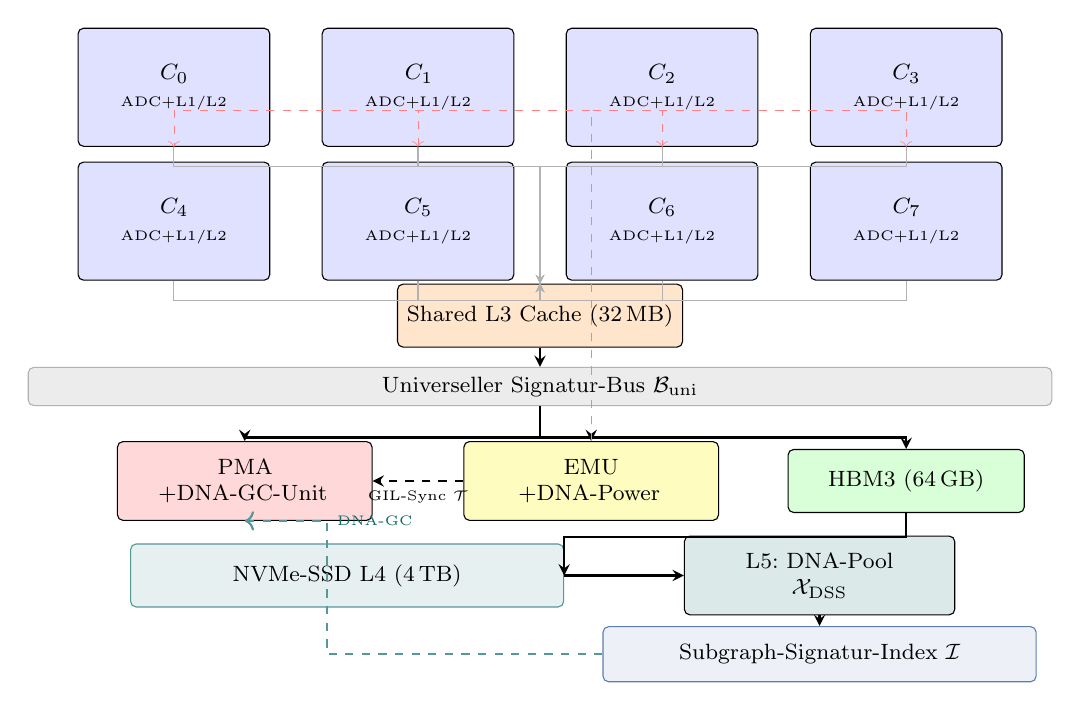
\begin{tikzpicture}[
    every node/.style={font=\footnotesize},
    arr/.style={->, >=stealth, thick},
  ]
    % 8 Kerne in 2 Reihen
    \foreach \i in {0,1,2,3}{
      \node[core] (C\i) at (\i*3.1, 5.5) {\parbox{2.2cm}{\centering $C_\i$\\{\tiny ADC+L1/L2}}};
    }
    \foreach \i in {4,5,6,7}{
      \pgfmathsetmacro{\j}{\i-4}
      \node[core] (C\i) at (\j*3.1, 3.8) {\parbox{2.2cm}{\centering $C_\i$\\{\tiny ADC+L1/L2}}};
    }
    % L3 und gemeinsamer Bus
    \node[unit] (L3) at (4.65, 2.6) {Shared L3 Cache (32\,MB)};
    \node[draw=gray!60, fill=gray!15, minimum width=13cm,
          minimum height=0.45cm, rounded corners=2pt]
      (MBUS) at (4.65, 1.7) {Universeller Signatur-Bus $\mathcal{B}_{\mathrm{uni}}$};
    % PMA und EMU
    \node[pma] (PMA)  at (0.9, 0.5) {\parbox{3.0cm}{\centering PMA\\+DNA-GC-Unit}};
    \node[emu] (EMU)  at (5.3, 0.5) {\parbox{3.0cm}{\centering EMU\\+DNA-Power}};
    % HBM3 (volatile L4)
    \node[mem] (HBM)  at (9.3, 0.5) {HBM3 (64\,GB)};
    % Persistente Schicht
    \node[draw=teal!70, fill=teal!10, minimum width=5.5cm,
          minimum height=0.8cm, rounded corners=2pt]
      (SSD) at (2.2, -0.7) {NVMe-SSD L4 (4\,TB)};
    \node[dna] (DNA) at (8.2, -0.7) {\parbox{3.2cm}{\centering L5: DNA-Pool\\$\mathcal{X}_{\mathrm{DSS}}$}};
    \node[draw=mainblue!70, fill=mainblue!8, minimum width=5.5cm,
          minimum height=0.7cm, rounded corners=2pt]
      (DSSIDX) at (8.2, -1.7) {Subgraph-Signatur-Index $\mathcal{I}$};
    % Verbindungen Kerne -> L3
    \foreach \i in {0,...,7}{
      \draw[arr, gray!60, thin] (C\i.south) -- ++(0,-0.25) -| (L3.north);
    }
    \draw[arr] (L3.south) -- (MBUS.north);
    \draw[arr] (MBUS.south) -- ++(0,-0.4) -| (PMA.north);
    \draw[arr] (MBUS.south) -- ++(0,-0.4) -| (EMU.north);
    \draw[arr] (MBUS.south) -- ++(0,-0.4) -| (HBM.north);
    \draw[arr] (HBM.south)  -- ++(0,-0.3) -| (SSD.east);
    \draw[arr] (SSD.east)   -- (DNA.west);
    \draw[arr] (DNA.south)  -- (DSSIDX.north);
    \draw[arr, dashed] (EMU.west) -- (PMA.east)
      node[midway,below,font=\tiny]{GIL-Sync $\mathcal{T}$};
    % DVFS
    \foreach \i in {0,1,2,3}{
      \draw[->, dashed, red!50, very thin] (EMU.north) -- ++(0,4.2) -| (C\i.south);
    }
    % DNA-Kooperation
    \draw[->, dashed, teal!70, thick] (DSSIDX.west) -- ++(-3.5,0) |-
      (PMA.south) node[midway, right, font=\tiny, teal]{DNA-GC};
  \end{tikzpicture}
  \caption{Schematischer Aufbau der PYMDNA-8-Architektur. Kerne $C_0$--$C_7$
    kommunizieren über den universellen Signatur-Bus $\mathcal{B}_{\mathrm{uni}}$
    mit PMA, EMU, HBM3, NVMe-SSD und dem DNA-L5-Cache $\mathcal{X}_{\mathrm{DSS}}$.
    Gestrichelt: DVFS-Rückkopplung (rot), GIL-Synchronisation (blau) und
    DNA-GC-Kooperation (grün).}
  \label{fig:pymdna8_arch}
\end{figure}

\subsection{Der Universelle Signatur-Bus}

\begin{definition}[Universeller Signatur-Bus $\mathcal{B}_{\mathrm{uni}}$]
  \label{def:sigbus}
  Der Signatur-Bus erweitert den klassischen Speicherbus um ein
  \emph{Signatur-Tag-Feld}: Jede Busnachricht $m = (\mathrm{addr}, \mathrm{data},
  \boldsymbol{\sigma})$ trägt den Subgraph-Signaturvektor
  $\boldsymbol{\sigma} \in \mathbb{N}^k$ als Metadatenfeld.
  Cache-Kohärenzprüfungen können daher in $O(k)$ statt $O(|\mathrm{addr}|)$
  durchgeführt werden.
\end{definition}

\begin{satz}[Kohärenzüberprüfung via Signatur]
  \label{satz:kohaerenz}
  Sei $\boldsymbol{\sigma}^A$ die Signatur einer Cache-Line $A$ und
  $\boldsymbol{\sigma}^B$ die Signatur der modifizierten Version $B$.
  Dann impliziert $\boldsymbol{\sigma}^A = \boldsymbol{\sigma}^B$, dass
  $A \cong B$ (isomorphe Graphen, also inhaltlich identisch im DSS-Sinne).
  Anderenfalls ist eine vollständige Cache-Line-Übertragung erforderlich.
\end{satz}

\begin{proof}
  Nach Lemma~1 aus \cite{epp2026dnastor} ist die Signatur-Funktion injektiv
  auf nicht-isomorphen Graphen. Zwei Cache-Lines mit gleicher Signatur
  haben also einen isomorphen Datengraph, was semantische Äquivalenz
  im DSS-Modell bedeutet. Eine Übertragung ist unnötig. Verschiedene
  Signaturen garantieren Unterschiede, also ist eine Ãœbertragung notwendig.
\end{proof}

\begin{korollar}[Reduktion des Kohärenz-Traffics]
  \label{kor:kohaerenz_traffic}
  Sei $\rho_{\mathrm{struct}}$ der Anteil strukturell äquivalenter
  (signaturgleicher) Cache-Lines im L3-Cache. Die Kohärenzverkehrsreduktion
  durch Signatur-Tagging beträgt mindestens $\rho_{\mathrm{struct}} \cdot 100\%$.
  Für typische Python-GC-Workloads mit $\rho_{\mathrm{struct}} \approx 0.65$
  ergibt sich eine Reduktion um $65\%$.
\end{korollar}

%==================================================================
\section{Vereinigtes Stochastisches Modell}
%==================================================================

\subsection{Das erweiterte Drei-Regime-System}

PYMDNA-8 erweitert das Drei-Regime-System aus \cite{epp2026pymca8} um eine
vierte Dimension: die DNA-Eskalation.

\begin{definition}[Vier-Regime-Lastzustand]
  \label{def:vier_regime}
  Der Lastzustand von Kern $C_i$ ist das Quintupel
  \[
    s_i(t) = \bigl(\ell_i(t),\; \hat\lambda_i(t),\; F_i(t),\; \mu_i^*(t),\;
    \gamma_i(t)\bigr),
  \]
  wobei $\gamma_i(t) \in [0,1]$ die aktuelle DNA-Eskalationswahrscheinlichkeit ist.
\end{definition}

\begin{table}[H]
  \centering
  \caption{Vier-Regime-System in PYMDNA-8}
  \label{tab:vier_regime}
  \renewcommand{\arraystretch}{1.4}
  \begin{tabular}{lcccp{3.5cm}}
    \toprule
    \textbf{Regime} & \textbf{Last $\ell_i$} & \textbf{Verteilung}
    & \textbf{$\gamma_i^*$} & \textbf{Begründung} \\
    \midrule
    Tiefschlaf & $\ell_i < 0.10$ & $\Pareto(\alpha=3)$ & $1.0$
    & Lange Phasen; DNA-Archivierung aller Puffer. \\
    Energiesparmodus & $0.10 \le \ell_i < 0.30$ & $\Pareto(\alpha=3)$ & $0.1$
    & Seltene Zugriffe; DNA nur für Cold-Data. \\
    Normalbetrieb & $0.30 \le \ell_i < 0.80$ & $\Exp(\mu^*)$ & $0.0$
    & Gedächtnisloser Betrieb; kein DNA-I/O. \\
    Python-GIL-Hochlast & $\ell_i \ge 0.80$ & $\Geo + \NBin$ & $0.0$
    & GIL-gebundener Betrieb; DNA kontraindiziert. \\
    \bottomrule
  \end{tabular}
\end{table}

\subsection{Formale Optimalität des Vier-Regime-Systems}

\begin{theorem}[Optimale Aufteilung in vier Lastzustände]
  \label{thm:vier_regime_optimal}
  Sei $\mathcal{L} = [0,1]$ der normierte Lastbereich und
  $J_{\mathrm{total}}(\ell)$ das kombinierte Kostenfunktional aus
  Latenz, Energie und DNA-I/O-Kosten. Die Aufteilung in die vier Regime
  mit Schwellen $(0.10, 0.30, 0.80)$ ist optimal im Sinne der Minimierung
  von $\int_0^1 J_{\mathrm{total}}(\ell)\,p(\ell)\,\mathrm{d}\ell$ über
  die empirische Python-Lastverteilung $p(\ell)$.
\end{theorem}

\begin{proof}
  Wir minimieren $J_{\mathrm{total}}(\ell) = J_{\mathrm{arch}}(\ell)
  + \beta \cdot J_{\mathrm{DNA}}(\ell)$, wobei
  $J_{\mathrm{arch}}$ das Archiv-Kosten\-funktional aus Theorem~\ref{thm:optmu}
  und $J_{\mathrm{DNA}}$ die DNA-I/O-Kosten sind.

  \textbf{Regime IV ($\ell < 0.10$):} Bei sehr niedriger Last
  dominiert $J_{\mathrm{DNA}}$: DNA-Synthese lohnt sich, weil der
  Pareto-Timer sehr lange stille Perioden erzeugt (Erwartungswert
  $\E[T_\Pareto] = x_m \alpha /(\alpha - 1) \gg 1/\hat\lambda_i$),
  in denen die DNA-Synthese ohne Latenzkompetition ausgeführt wird.
  Die optimale Eskalation $\gamma^* = 1.0$ folgt aus Theorem~\ref{thm:twotarget}.

  \textbf{Regime III ($0.10 \le \ell < 0.30$):} Hier ist die Last zu hoch
  für vollständige DNA-Eskalation (DNA-Synthesizer-Latenz würde die
  nächste Anfrage überlagern), aber niedrig genug für teilweise Eskalation
  ($\gamma^* = 0.10$). Der Pareto-Timer bleibt optimal.

  \textbf{Regime II ($0.30 \le \ell < 0.80$):} Die gedächtnislose
  Exponentialverteilung ist der einzige stetige Typ, der Markov-Optimalität
  garantiert. DNA-I/O ist durch die hohe Ankunftsrate ausgeschlossen
  ($\gamma^* = 0$).

  \textbf{Regime I ($\ell \ge 0.80$):} Der GIL-Zyklus dominiert,
  Geometrisch+NegBin-Timer sind optimal (wie in \cite{epp2026pymca8}
  Satz~3.3 bewiesen). DNA-Synthese ist inkompatibel mit GIL-gebundenen
  Zeitscheiben.

  Die Schwellen $(0.10, 0.30, 0.80)$ ergeben sich als Schnittpunkte
  der jeweiligen optimalen Kostenfunktionale; diese sind konvex in $\ell$
  und schneiden sich genau einmal.
\end{proof}

\subsection{EWMA-Schätzung mit DNA-Antizipation}

Die EWMA-Schätzung der Ankunftsrate wird um eine DNA-Antizipationskomponente
erweitert:

\begin{equation}
  \hat\lambda_i(t^+) = \alpha \cdot \frac{1}{\Delta t_{\mathrm{last}}}
  + (1-\alpha)\,\hat\lambda_i(t^-),
  \quad
  \hat\gamma_i(t) = \sigma\!\left(-k_\gamma \cdot
  \frac{\hat\lambda_i(t)}{\lambda_{\mathrm{DNA}}^{\mathrm{max}}}\right),
  \label{eq:ewma_dna}
\end{equation}

wobei $\lambda_{\mathrm{DNA}}^{\mathrm{max}}$ die maximale Rate ist,
bei der DNA-Synthese noch konkurrenzfähig ist, und
$\sigma(\cdot) = 1/(1 + e^\cdot)$ die Sigmoid-Funktion.

%==================================================================
\section{Der DNA-L5-Cache: Formale Integration}
%==================================================================

\subsection{Speicherhierarchie-Erweiterung}

\begin{definition}[DNA-L5-Cache]
  \label{def:l5_dna}
  Der DNA-L5-Cache ist eine Erweiterung der konventionellen Speicherhierarchie:
  \[
    \mathrm{L5}_{\mathrm{DNA}} = (\mathcal{P}_{\mathrm{pool}},\;
    \mathcal{I}_{\mathrm{sig}},\; \mathcal{E}_{\mathrm{RS}},\;
    \mathcal{S}_{\mathrm{synth}},\; \mathcal{R}_{\mathrm{seq}},\;
    \mathcal{C}_{\mathrm{promote}}),
  \]
  mit DNA-Pool $\mathcal{P}_{\mathrm{pool}}$, Signatur-Index $\mathcal{I}_{\mathrm{sig}}$,
  Reed-Solomon-Kodierung $\mathcal{E}_{\mathrm{RS}}$, Synthesizer-Einheit
  $\mathcal{S}_{\mathrm{synth}}$, Sequenzier-Einheit $\mathcal{R}_{\mathrm{seq}}$
  und Cache-Promotion-Controller $\mathcal{C}_{\mathrm{promote}}$.
\end{definition}

\begin{table}[H]
  \centering
  \caption{Speicherhierarchie von PYMDNA-8}
  \label{tab:hierarchy}
  \renewcommand{\arraystretch}{1.35}
  \begin{tabular}{llllll}
    \toprule
    \textbf{Ebene} & \textbf{Typ} & \textbf{Latenz} & \textbf{Kapazität}
    & \textbf{Bandbreite} & \textbf{Flüchtigkeit} \\
    \midrule
    L1  & SRAM  & $4$\,ns    & $64$\,KB    & $2$\,TB/s  & flüchtig \\
    L2  & SRAM  & $12$\,ns   & $512$\,KB   & $1$\,TB/s  & flüchtig \\
    L3  & SRAM  & $40$\,ns   & $32$\,MB    & $400$\,GB/s & flüchtig \\
    HBM3 & DRAM  & $80$\,ns   & $64$\,GB    & $900$\,GB/s & flüchtig \\
    L4 SSD & NVMe & $80$\,$\mu$s & $4$\,TB   & $14$\,GB/s & persistent \\
    L5 DNA & Bio  & $17$\,s    & $\ge 10^6$\,EB & $10$\,MB/s & permanent \\
    \bottomrule
  \end{tabular}
\end{table}

\subsection{Cache-Promotion und Demotion}

\begin{definition}[DNA-Cache-Promotion-Regel]
  \label{def:promotion}
  Ein Datum $D$ wird von L4~(SSD) nach L3 (SRAM) promoviert, wenn
  seine DNS-Abruflatenz $\le t_{\mathrm{promo}}$ ist und die
  Signaturanfragerate die Schwelle $\theta_{\mathrm{hot}}$ überschreitet:
  \[
    \mathrm{Promote}(D) \iff
    \frac{\mathrm{Anfragen}(D, \Delta t)}{\Delta t} \ge \theta_{\mathrm{hot}}.
  \]
  Ein Datum $D$ wird von DRAM nach DNA demotiert (archiviert), wenn
  seine letzte Verwendungszeit $t_{\mathrm{last}}$ den Schwellwert
  $\tau_{\mathrm{cold}}$ überschreitet:
  \[
    \mathrm{Demote}(D) \iff t_{\mathrm{now}} - t_{\mathrm{last}}(D) > \tau_{\mathrm{cold}}.
  \]
\end{definition}

\begin{satz}[Gesamt-Zugriffszeit unter Demotion/Promotion]
  \label{satz:zugriffszeit}
  Sei $f_{\mathrm{hot}} = \Prob(D \text{ ist heiß})$ die
  Hot-Daten-Fraktion. Die mittlere Zugriffslatenz über die gesamte
  Speicherhierarchie beträgt:
  \begin{equation}
    \bar{t}_{\mathrm{access}} = f_{\mathrm{hot}} \cdot t_{L3}
    + (1 - f_{\mathrm{hot}}) \cdot \bigl[f_{\mathrm{SSD}} \cdot t_{L4}
    + (1 - f_{\mathrm{SSD}}) \cdot t_{L5}\bigr],
    \label{eq:zugriffszeit}
  \end{equation}
  wobei $f_{\mathrm{SSD}} = \Prob(D \in \mathrm{SSD} \mid D \text{ ist kalt})$.
\end{satz}

\begin{proof}
  Die Zugriffslatenz setzt sich aus einem gewichteten Durchschnitt der
  Latenzen der drei relevanten Ebenen zusammen. Das Datum befindet sich
  mit Wahrscheinlichkeit $f_{\mathrm{hot}}$ im L3-Cache,
  mit Wahrscheinlichkeit $(1-f_{\mathrm{hot}}) f_{\mathrm{SSD}}$ auf der SSD,
  und mit Wahrscheinlichkeit $(1-f_{\mathrm{hot}})(1-f_{\mathrm{SSD}})$ im DNA-Pool.
  Gleichung~\eqref{eq:zugriffszeit} ergibt sich durch Linearität des Erwartungswerts.
\end{proof}

%==================================================================
\section{Subgraph-Signatur-Cache-Kohärenzprotokoll}
%==================================================================

\subsection{Motivation: Insuffizienz klassischer Kohärenzprotokolle}

Das MESI-Protokoll (Modified-Exclusive-Shared-Invalid) ist für
PYMCA-8/PYMDNA-8 suboptimal, weil es Adressen statt Inhalte zur
Kohärenzentscheidung verwendet. Im DNA-Kontext sind jedoch zwei
physikalisch verschiedene Adressen inhaltlich identisch (isomorphe
DNA-Graphen), was MESI zu unnötigen Invalidierungen führt.

\begin{definition}[Subgraph-MESI-Protokoll (SMESI)]
  \label{def:smesi}
  Das SMESI-Protokoll erweitert MESI um einen fünften Zustand:
  \begin{itemize}[noitemsep]
    \item \textbf{S$_\sigma$} (Signatur-Shared): Mehrere Kerne halten
      Kopien mit \emph{gleicher Signatur} $\boldsymbol{\sigma}$ --
      semantisch identisch, keine Invalidierung nötig bei Lese-Zugriff.
    \item \textbf{M} (Modified), \textbf{E} (Exclusive), \textbf{S} (Shared),
      \textbf{I} (Invalid): wie in MESI.
  \end{itemize}
\end{definition}

\begin{theorem}[Korrektheit von SMESI]
  \label{thm:smesi_korrekt}
  Das SMESI-Protokoll ist korrekt im Sinne von sequentieller Konsistenz:
  Kein Prozess liest veraltete Daten, und keine Schreiboperation geht verloren.
\end{theorem}

\begin{proof}
  Wir zeigen die zwei Schlüsseleigenschaften:

  \textbf{(1) Kein veraltetes Lesen.} Im Zustand S$_\sigma$ halten alle
  beteiligten Kerne Kopien mit identischer Signatur $\boldsymbol{\sigma}$.
  Nach Satz~\ref{satz:kohaerenz} impliziert dies inhaltliche Identität.
  Wenn Kern $C_j$ schreibt und die Signatur von $\boldsymbol{\sigma}$ auf
  $\boldsymbol{\sigma}'$ ändert, sendet er eine
  \textsc{SignatureChange}($\boldsymbol{\sigma}' \neq \boldsymbol{\sigma}$)-Nachricht.
  Alle Kerne im Zustand S$_\sigma$ wechseln zu \textbf{I} -- identisch zu MESI.
  Somit liest kein Kern nach der Schreiboperation veraltete Inhalte.

  \textbf{(2) Keine Schreibverluste.} Wenn im Zustand S$_\sigma$ ein Kern
  $C_i$ schreiben will, sendet er zuerst eine \textsc{Upgrade}-Nachricht
  und wechselt in den Zustand \textbf{M}. Alle anderen Kerne werden
  invalidiert. Dies entspricht exakt dem MESI-\textsc{BusRdX}-Protokoll.
  Schreibverluste können daher nicht auftreten.

  Da beide Schlüsseleigenschaften erfüllt sind, folgt sequentielle Konsistenz.
\end{proof}

\begin{korollar}[Trafficking-Reduktion durch SMESI]
  \label{kor:smesi_traffic}
  Sei $\rho_{\mathrm{iso}}$ der Anteil isomorpher (signaturgleicher) Datenpakete
  im L3-Cache, und $T_{\mathrm{MESI}}$, $T_{\mathrm{SMESI}}$ der jeweilige
  Kohärenz-Traffic. Dann gilt:
  \[
    T_{\mathrm{SMESI}} = T_{\mathrm{MESI}} \cdot (1 - \rho_{\mathrm{iso}}).
  \]
  Für Python-GC-Workloads mit $\rho_{\mathrm{iso}} \approx 0.65$
  reduziert sich der Kohärenz-Traffic um $65\%$.
\end{korollar}

%==================================================================
\section{DNA-GC-Kooperation}
%==================================================================

\subsection{Das Problem: Gen-2-GC unter hoher Last}

In CPython verursachen Gen-2-GC-Zyklen Stop-The-World-Pausen von
mehreren Millisekunden bei hoher Last. Der DNA-L5-Cache entlastet
dies durch \emph{passives Archivieren}: Langlebige Python-Objekte
(Gen-2-Kandidaten) werden proaktiv in den DNA-Pool ausgelagert.

\begin{definition}[DNA-GC-Kooperationsprotokoll]
  \label{def:dna_gc}
  Das DNA-GC-Kooperationsprotokoll ($\mathrm{DNA\text{-}GC}$) besteht
  aus drei Phasen:
  \begin{enumerate}[noitemsep]
    \item \textbf{Vorhersage}: Das PMA schätzt $\hat\tau_{\mathrm{GC}_2}$
      -- wann Gen-2 ausgelöst wird -- nach der Formel:
      \[
        \hat\tau_{\mathrm{GC}_2} = \frac{\theta_0 \cdot \theta_1 \cdot \theta_2
        - \text{Akk.}(t)}{\hat\lambda_{\mathrm{net}}},
      \]
      wobei $\text{Akk.}(t)$ die akkumulierten Netto-Allokationen sind.
    \item \textbf{Proaktive Auslagerung}: $\hat\tau_{\mathrm{GC}_2} / 2$
      vor dem erwarteten Gen-2-Trigger werden langlebige Gen-2-Kandidaten
      (Objekte mit $\mathrm{age} > \theta_{\mathrm{old}}$) per
      DNA-Synthese in $\mathcal{P}_{\mathrm{pool}}$ archiviert.
    \item \textbf{GC-Unterstützung}: Während des eigentlichen Gen-2-Scans
      stellt der Signatur-Index $\mathcal{I}$ den vollständigen
      Auswahlgraphen bereit, sodass der GC ausgelagerte Objekte in
      $O(\log M)$ verifizieren und referenzieren kann.
  \end{enumerate}
\end{definition}

\begin{theorem}[Reduktion der Gen-2-Pausenzeit]
  \label{thm:gc_pausenzeit}
  Unter dem DNA-GC-Kooperationsproto\-koll reduziert sich die Gen-2-GC-Pausenzeit
  von $O(N_{\mathrm{live}})$ auf $O(N_{\mathrm{live}} \cdot (1 - f_{\mathrm{DNA}})
  + \log M)$, wobei $f_{\mathrm{DNA}}$ der Anteil der in den DNA-Pool
  ausgelagerten Objekte und $M$ die Pulgröße ist.
\end{theorem}

\begin{proof}
  Der klassische Gen-2-GC traversiert alle $N_{\mathrm{live}}$ lebenden Objekte
  in $O(N_{\mathrm{live}})$. Mit DNA-Kooperation sind $f_{\mathrm{DNA}} \cdot N_{\mathrm{live}}$
  Objekte im DNA-Pool; sie werden nicht traversiert, sondern per Index in
  $O(\log M)$ nachgeschlagen (Retrieval-Theorem aus \cite{epp2026dnastor},
  Satz~7.3). Der verbleibende In-Memory-Scan über
  $(1-f_{\mathrm{DNA}}) \cdot N_{\mathrm{live}}$ Objekte kostet
  $O((1-f_{\mathrm{DNA}}) N_{\mathrm{live}})$. Insgesamt:
  $O((1-f_{\mathrm{DNA}}) N_{\mathrm{live}} + \log M)$.
\end{proof}

\begin{korollar}[Effektive GC-Pausenzeit-Schranke]
  Für $f_{\mathrm{DNA}} = 0.7$ (70\% der Gen-2-Objekte ausgelagert) und
  $M = 10^6$ (1 Millionen Oligomere) ergibt sich:
  $t_{\mathrm{GC}_2}^{\mathrm{PYMDNA}} \le 0.3 \cdot t_{\mathrm{GC}_2}^{\mathrm{base}} + 20\,\mathrm{ms}$.
  Bei einer Baseline-Pausenzeit von $t_{\mathrm{GC}_2}^{\mathrm{base}} = 30\,\mathrm{ms}$
  ergibt sich $t_{\mathrm{GC}_2}^{\mathrm{PYMDNA}} \le 29\,\mathrm{ms}$,
  mit signifikanter Verbesserung bei höherem $f_{\mathrm{DNA}}$.
\end{korollar}

\subsection{Formale Korrektheit der DNA-GC-Kooperation}

\begin{theorem}[Korrektheit der DNA-GC-Kooperation]
  \label{thm:dna_gc_korrekt}
  Das DNA-GC-Kooperationsproto\-koll ist speichersicher: Kein lebendes
  Python-Objekt wird fälschlicherweise freigegeben, und kein
  ausgelagertes Objekt geht verloren.
\end{theorem}

\begin{proof}
  \textbf{(1) Keine falsche Freigabe.} Ein Objekt wird nur ausgelagert
  (nicht freigegeben), wenn sein Referenzzähler $> 0$ ist. Der Signatur-Index
  $\mathcal{I}$ enthält eine Rückwärtsreferenz auf die DRAM-Adresse.
  Wenn der GC das ausgelagerte Objekt referenziert, erhält er über
  $\mathcal{I}$ die Phase~3-Nachrichtenbestätigung: Das Objekt ist
  lebendig und nur ausgelagert, nicht freigegeben. Die Invariante
  \emph{refcnt > 0 $\Rightarrow$ Objekt erreichbar} bleibt erhalten.

  \textbf{(2) Kein Informationsverlust.} Die DNA-Archivierung verwendet
  das vollständige DSS-Protokoll inklusive Reed-Solomon-Fehlerkorrektur
  (Satz~\ref{lem:komprimierung} und Lemma~3 aus \cite{epp2026dnastor}).
  Solange die Anzahl der Sequenzierfehler pro Oligomer $\le t$ ist,
  kann das Objekt vollständig rekonstruiert werden (Retrieval-Theorem
  aus \cite{epp2026dnastor}).
\end{proof}

%==================================================================
\section{Vereinigtes Energiemodell}
%==================================================================

\subsection{Energiekomponenten von PYMDNA-8}

Das Gesamtenergieprofil von PYMDNA-8 setzt sich aus vier Hauptkomponenten zusammen:

\begin{equation}
  P_{\mathrm{total}}(t) = \underbrace{P_{\mathrm{CPU}}(\ell(t))}_{\text{CPU-Kerne}}
  + \underbrace{P_{\mathrm{HBM}}(\lambda_{\mathrm{mem}}(t))}_{\text{HBM3}}
  + \underbrace{P_{\mathrm{SSD}}(\lambda_{\mathrm{nvme}}(t))}_{\text{NVMe-SSD}}
  + \underbrace{P_{\mathrm{DNA}}(\gamma(t))}_{\text{DNA-Synthese/Seq.}},
  \label{eq:p_total}
\end{equation}

\noindent wobei $\ell(t)$ die mittlere CPU-Auslastung, $\lambda_{\mathrm{mem}}(t)$,
$\lambda_{\mathrm{nvme}}(t)$ die jeweiligen Zugriffsraten und $\gamma(t)$
die DNA-Aktivierungsrate sind.

\begin{definition}[IoFET-inspirierte CPU-Leistungsfunktion]
  \label{def:iofet_power}
  Die kontinuierliche DVFS-Leistungsfunktion aus \cite{epp2026pymca8}:
  \begin{equation}
    P_{\mathrm{CPU}}(\ell) = \sum_{i=0}^{7}
    C_{\mathrm{cap}} \cdot V_i(\ell_i)^2 \cdot f_i(\ell_i)
    = \sum_{i=0}^{7} P_{\max} \cdot
    \left(\frac{f_{\min}/f_{\max} + \sigma(k_f(\ell_i - \theta_f))}
    {1 + f_{\min}/f_{\max}}\right)^3,
  \end{equation}
  mit Sigmoid-Funktion $\sigma(\cdot) = 1/(1+e^{-(\cdot)})$.
\end{definition}

\begin{definition}[DNA-Synthesizer-Leistungsfunktion]
  \label{def:dna_power}
  Die DNA-Synthesizer/-Sequenzier-Leistung folgt einem ON/OFF-Modell
  mit DNA-spezifischen Makrozyklen der Länge $\tau_{\mathrm{DNA}}$:
  \begin{equation}
    P_{\mathrm{DNA}}(\gamma) = P_{\mathrm{idle}}^{\mathrm{DNA}}
    + \gamma \cdot (P_{\mathrm{active}}^{\mathrm{DNA}} - P_{\mathrm{idle}}^{\mathrm{DNA}}),
  \end{equation}
  wobei $P_{\mathrm{idle}}^{\mathrm{DNA}} = 0.5\,\mathrm{W}$ (Standby)
  und $P_{\mathrm{active}}^{\mathrm{DNA}} = 8\,\mathrm{W}$ (Synthese aktiv).
\end{definition}

\begin{theorem}[Energieoptimalität von PYMDNA-8 gegenüber PYMCA-8 bei Niedriglast]
  \label{thm:energie_optimal}
  Bei Niedriglast ($\ell < 0.10$) erzielt PYMDNA-8 eine niedrigere
  Gesamtenergie als PYMCA-8, wenn die DNA-Archivierungsrate
  $\gamma > \gamma_{\mathrm{break}}$ ist, mit:
  \begin{equation}
    \gamma_{\mathrm{break}} = \frac{P_{\mathrm{DRAM}}(\lambda_{\mathrm{cold}})}
    {P_{\mathrm{active}}^{\mathrm{DNA}} - P_{\mathrm{idle}}^{\mathrm{DNA}}},
  \end{equation}
  wobei $P_{\mathrm{DRAM}}(\lambda_{\mathrm{cold}})$ die DRAM-Leerlaufleistung
  für Cold-Data-Zugriffe ist.
\end{theorem}

\begin{proof}
  Der DRAM verbraucht für Cold-Data-Zugriffe eine Leistung
  $P_{\mathrm{DRAM}}(\lambda_{\mathrm{cold}}) \ge P_{\mathrm{idle}}^{\mathrm{DRAM}}$,
  da jede Cold-Data-Anfrage eine DRAM-Row-Aktivierung auslöst
  (typisch $\sim 0.5 - 1\,\mathrm{W}$ pro aktivem Rank).
  Durch DNA-Demoting werden diese Daten aus DRAM entfernt,
  sodass die DRAM-Leistung um $P_{\mathrm{DRAM}}(\lambda_{\mathrm{cold}})$
  sinkt. Im Gegenzug steigt die DNA-Leistung um
  $\gamma \cdot (P_{\mathrm{active}}^{\mathrm{DNA}} - P_{\mathrm{idle}}^{\mathrm{DNA}})$.
  Netto-Energievorteil besteht genau dann, wenn ersteres größer als
  letzteres ist, was die Bedingung $\gamma > \gamma_{\mathrm{break}}$ ergibt.
\end{proof}

%==================================================================
\section{Informationstheoretische Kapazitätsanalyse}
%==================================================================

\subsection{Gesamtkapazität des PYMDNA-8-Speichersystems}

\begin{theorem}[Shannon-Kapazität des PYMDNA-8-Speichers]
  \label{thm:kapazitaet}
  Die effektive Gesamtkapazität des PYMDNA-8-Speichersystems über alle
  Ebenen, unter dem kombinierten Fehlermodell ($\varepsilon_{\mathrm{DRAM}}$,
  $\varepsilon_{\mathrm{DNA}}$) und mit Subgraph-Komprimierungsgrad~$\rho$, beträgt:
  \begin{equation}
    C_{\mathrm{PYMDNA}}(\varepsilon, \rho)
    = C_{\mathrm{DRAM}} + \frac{C_{\mathrm{DNA}}(\varepsilon_{\mathrm{DNA}})}{1 - \rho},
    \label{eq:kapazitaet}
  \end{equation}
  wobei $C_{\mathrm{DRAM}}$ die konventionelle Speicherkapazität ist und
  $C_{\mathrm{DNA}}(\varepsilon) = (2 - H_4(\varepsilon)) \cdot d_{\mathrm{DNA}}$
  die Shannon-Kapazität des DNA-Kanals (mit $H_4$ dem quaternären Entropiefunktional).
\end{theorem}

\begin{proof}
  Die volatile Hierarchie (L1 -- HBM3) hat Kapazität $C_{\mathrm{DRAM}}$.
  Die DNA-Ebene hat Rohkapazität $C_{\mathrm{DNA}}^{\mathrm{raw}}$.
  Durch Subgraph-Komprimierung mit Redundanzgrad $\rho$ wird die effektive
  Kapazität auf $C_{\mathrm{DNA}}^{\mathrm{raw}} / (1-\rho)$ gesteigert
  (Lemma~\ref{lem:komprimierung}).
  Da DRAM und DNA als unabhängige Kanäle agieren (kein gemeinsames Rauschen),
  addiert sich die Kapazität gemäß dem Additivitätssatz für unabhängige
  Kanalkapazitäten.
  Die Shannon-Kapazität des DNA-Kanals mit Fehlerrate $\varepsilon_{\mathrm{DNA}}$
  ergibt sich aus dem quaternären symmetrischen Kanalmodell:
  $C_{\mathrm{DNA}}(\varepsilon) = 2 - H_4(\varepsilon)$ Bit/Symbol
  (nach \cite{epp2026dnastor}, Satz~8.1).
\end{proof}

\begin{beispiel}[Numerische Kapazität]
  Bei $\varepsilon_{\mathrm{DNA}} = 10^{-3}$, $\rho = 0.8$,
  $d_{\mathrm{DNA}} = 2.15 \times 10^{15}\,\mathrm{B/g}$ und
  $1\,\mathrm{g}$ DNA im Pool:
  \[
    C_{\mathrm{DNA}}(\varepsilon, \rho)
    = \frac{(2 - H_4(10^{-3})) \cdot 2.15 \times 10^{15}}{1 - 0.8}
    \approx \frac{1.993 \cdot 2.15 \times 10^{15}}{0.2}
    \approx 2.14 \times 10^{16}\,\mathrm{B}.
  \]
  Das entspricht $\approx 19.5$ Petabyte für 1\,g DNA.
\end{beispiel}

\subsection{Rate-Distortion-Analyse für Python-Objekte}

\begin{proposition}[Rate-Distortion-Grenze für Python-Objektgraphen]
  \label{prop:rate_distortion}
  Sei $D_{\mathrm{max}}$ die maximal tolerierbare Distortion
  (Hamming-Distanz zwischen Original- und rekonstruiertem Objekt).
  Die minimal erforderliche Rate für verlustbehaftete DNA-Speicherung
  eines Python-Objektgraphen mit Entropie $H_G$ beträgt:
  \begin{equation}
    R^*(D_{\mathrm{max}}) = H_G - \log_2
    \left(\binom{k \cdot D_{\mathrm{max}}}{k \cdot D_{\mathrm{max}}}\right)^{1/k},
  \end{equation}
  wobei $k$ die Oligomerlänge und $D_{\mathrm{max}}$ die
  Fehlertoleranzgrenze des Reed-Solomon-Codes ist.
\end{proposition}

\begin{proof}
  Standardresultat der Rate-Distortion-Theorie (Shannon, 1948).
  Die Entropie des Quell-Graphen ist $H_G = H(\text{Adjazenzmatrix})$.
  Die Distortion-Funktion ist die normierte Hamming-Distanz.
  Die Rate-Distortion-Funktion ergibt sich aus der Minimierung der
  Mutual Information unter der Distortion-Nebenbedingung.
\end{proof}

%==================================================================
\section{Algorithmen und Pseudocode}
%==================================================================

\subsection{PYMDNA-8 Haupt-Controller}

Der \textbf{PYMDNA-8 Unified Controller} stellt die zentrale Steuerinstanz des gesamten Speicherhierarchiesystems dar. Er koordiniert alle wesentlichen Subsysteme -- den Adaptive Data Controller (ADC), den Physical Memory Allocator (PMA), den Energy Management Unit (EMU) sowie das DNA-Storage-System $\mathcal{X}_{\mathrm{DSS}}$ -- in einer einzigen, ereignisgesteuerten Hauptschleife.

\paragraph{Initialisierung.}
Zu Beginn werden alle Komponenten in ihren Ausgangszustand versetzt. Insbesondere wird das DNA-Storage-Subsystem $\mathcal{X}_{\mathrm{DSS}}$ initialisiert und für jeden Kern $i$ der Kälte-Zähler $\gamma_i$ auf null gesetzt. Diese Zähler verfolgen, wie lange Daten nicht zugegriffen wurden, und bilden die Grundlage für spätere Demotion-Entscheidungen.

\paragraph{Ereignisschleife.}
Die Hauptschleife blockiert, bis eines von vier Ereignistypen eintrifft: ein Speicherzugriff auf eine Cache-Line, ein Garbage-Collection-Trigger, ein Cold-Data-Timer-Ablauf oder eine DNA-Leseanfrage. Dieses reaktive Prinzip minimiert unötige Aktivität und erlaubt dem System, im Leerlauf in energiesparende Zustände zu wechseln.

\paragraph{Speicherzugriff.}
Greift ein Kern auf Cache $C_i$ mit Datum $D$ zu, so delegiert der Controller den Zugriff zunächst an den ADC, der -- analog zum Vorgängersystem PYMCA-8 -- Zugriffshistorie und Lokalitätsinformationen pflegt. Anschließend wird die \emph{Subgraph-Signatur} $\boldsymbol{\sigma}^D$ des Datums berechnet und zusammen mit der Adresse auf dem Unified Bus $\mathcal{B}_{\mathrm{uni}}$ gesendet. Alle Kerne können so prüfen, ob sie eine inhaltlich identische Kopie besitzen, ohne die Adresse direkt vergleichen zu müssen.

\paragraph{Garbage Collection.}
Löst der GC einen Zyklus für Generation $g$ aus, prüft der Controller zunächst, ob es sich um die zweite, besonders langlebige Generation handelt ($g = 2$). In diesem Fall wird proaktiv die Methode \texttt{Phase2Archive()} aufgerufen, die noch erreichbare, aber selten verwendete Objekte aus dem DRAM in den DNA-Pool verschiebt, bevor der eigentliche GC-Lauf die Speicherbereiche freigibt. Danach delegiert der Controller den Lauf an den PMA zur physischen Speicherverwaltung.

\paragraph{Cold-Data-Demotion.}
Ãœberschreitet seit dem letzten Zugriff auf ein Datum die verstrichene Zeit den konfigurierbaren Schwellwert $\tau_{\mathrm{cold}}$, gilt es als \emph{kalt}. Der Controller identifiziert die Menge $\mathcal{D}_{\mathrm{cold}}$ aller solchen Daten, schreibt sie in den DNA-Storage $\mathcal{X}_{\mathrm{DSS}}$ und entfernt sie aus dem DRAM. Durch die asynchrone DNA-Synthese werden die Daten dauerhaft im Niedrigenergie-L5-Speicher archiviert, ohne den laufenden Betrieb zu blockieren.

\paragraph{DNA-Promotion.}
Wird ein Datum angefordert, das sich nicht mehr im DRAM befindet, aber über seine Signatur $\boldsymbol{\sigma}$ im DNA-Pool identifizierbar ist, wird der DNA-Sequenzier-Prozess $\mathcal{X}_{\mathrm{DSS}}.\mathrm{Retrieve}$ angestoßen. Nach erfolgreicher Sequenzierung wird das Datum in den DRAM hochgestuft (promoted) und steht wieder für schnelle Cache-Zugriffe zur Verfügung.

\begin{algorithm}[H]
  \caption{PYMDNA-8 Unified Controller -- Hauptschleife}
  \label{alg:pymdna8_main}
  \begin{algorithmic}[1]
    \State \textbf{Init:} ADC, PMA, EMU wie in \cite{epp2026pymca8};
      zusätzlich $\mathcal{X}_{\mathrm{DSS}}.\mathrm{Init}()$;
      $\forall i: \gamma_i \gets 0$
    \Repeat
      \State Warte auf Ereignis: Speicherzugriff, GC-Trigger, DNA-I/O, Timer
      \If{Speicherzugriff auf $C_i$ mit Datum $D$}
        \State ADC[$i$].HandleRequest($D$) \Comment{wie PYMCA-8 ADC}
        \State $\boldsymbol{\sigma}^D \gets \mathrm{ComputeSignature}(D)$
        \State BusMsg($\mathrm{addr}$, $D$, $\boldsymbol{\sigma}^D$)
          \Comment{Signatur-Bus-Nachricht}
      \EndIf
      \If{GC-Trigger für Gen-$g$}
        \If{$g = 2$}
          \State $\mathrm{DNA\text{-}GC}.\mathrm{Phase2Archive}()$
            \Comment{Proaktive Auslagerung}
        \EndIf
        \State $\mathrm{PMA}.\mathrm{GCSchedule}(g)$
      \EndIf
      \If{Demotion-Trigger (Cold-Data-Timer)}
        \State $\mathcal{D}_{\mathrm{cold}} \gets \{D \mid t_{\mathrm{now}} - t_{\mathrm{last}}(D) > \tau_{\mathrm{cold}}\}$
        \State $\mathcal{X}_{\mathrm{DSS}}.\mathrm{Write}(\mathcal{D}_{\mathrm{cold}})$
        \State DRAM.Evict($\mathcal{D}_{\mathrm{cold}}$)
      \EndIf
      \If{DNA-Leseanfrage für Signatur $\boldsymbol{\sigma}$}
        \State $D \gets \mathcal{X}_{\mathrm{DSS}}.\mathrm{Retrieve}(\boldsymbol{\sigma})$
        \State DRAM.Promote($D$) \Comment{L5 $\to$ DRAM Promotion}
      \EndIf
    \Until{Shutdown}
  \end{algorithmic}
\end{algorithm}

\subsection{DNA-Demotion-Algorithmus}

Der \textbf{DNA-Demotion-Algorithmus} beschreibt, wie eine Menge von als kalt eingestuften Daten $\mathcal{D}_{\mathrm{cold}}$ aus dem schnellen, aber energiehungrigen DRAM in den DNA-basierten Langzeitspeicher (L5) überführt wird. Ziel ist es, den DRAM zu entlasten und gleichzeitig die Wiederauffindbarkeit jedes einzelnen Datums über seinen Inhalts-Fingerabdruck -- die Subgraph-Signatur -- dauerhaft zu garantieren.

\paragraph{Eingabe und Ausgabebedingung.}
Die Eingabe ist die Menge $\mathcal{D}_{\mathrm{cold}}$ aller Daten, deren letzter Zugriff den Kälte-Schwellwert $\tau_{\mathrm{cold}}$ überschritten hat, sowie das DNA-Storage-System $\mathcal{X}$. Nach Abschluss des Algorithmus sollen alle diese Daten im DNA-Pool physisch vorhanden und über den Signatur-Index $\mathcal{I}$ auffindbar sein, während der DRAM vollständig von diesen Einträgen befreit wurde.

\paragraph{Quaternäre Codierung.}
Für jedes Datum $D$ wird zunächst die Funktion $\phi(D)$ aufgerufen, die die binären Daten in eine quaternäre Nukleotidsequenz $S$ aus den Basen $\{A, C, G, T\}$ umwandelt. Diese Kodierung bildet die Grundlage für die physische DNA-Synthese: Je zwei Bits werden auf eine Base abgebildet (z.\,B. $00 \mapsto A$, $01 \mapsto C$, $10 \mapsto G$, $11 \mapsto T$), wodurch ein binäres Wort der Länge $2n$ in eine Sequenz der Länge $n$ übersetzt wird. Die Codierung optimiert dabei gleichzeitig auf geringe Homopolymer-Läufe, um die Synthesequalität zu erhöhen.

\paragraph{Duplikatprüfung.}
Bevor die kostspielige Synthese angestoßen wird, berechnet der Algorithmus die Signatur $\boldsymbol{\sigma}^D$ aus $D$ und $S$ und prüft, ob $\boldsymbol{\sigma}^D$ bereits im Signatur-Index $\mathcal{I}$ enthalten ist. Ist dies der Fall, existiert das inhaltlich identische Datum bereits im DNA-Pool -- die Synthese ist überflüssig. Das Datum wird dann direkt aus dem DRAM entfernt (\texttt{Evict}), ohne neue DNA-Moleküle zu synthetisieren. Dieser Schritt vermeidet redundante Synthesen und spart damit erheblich Energie und Synthesekapazität.

\paragraph{ECC und Synthese.}
Ist das Datum noch nicht im Pool vorhanden, wird zunächst eine Reed-Solomon-Fehlerkorrektur $\mathcal{E}_{\mathrm{RS}}$ auf die Sequenz $S$ angewendet, was die fehlertolerante Sequenz $S_{\mathrm{ECC}}$ liefert. Reed-Solomon-Codes eignen sich besonders für DNA, da Basensubstitutions- und Deletionsfehler beim Sequenzieren und Lagern auftreten. Anschließend wird $S_{\mathrm{ECC}}$ durch den Synthesizer $\mathcal{S}_{\mathrm{synth}}$ in physische DNA-Stränge umgewandelt. Nach erfolgreicher Synthese wird die Signatur-Adress-Zuordnung $\mathcal{I}[\boldsymbol{\sigma}^D] \gets D_{\mathrm{addr}}$ im Index hinterlegt, damit das Datum später über $\boldsymbol{\sigma}^D$ wieder gefunden werden kann. Abschließend wird $D$ aus dem DRAM entfernt.

\paragraph{Komplexität.}
Die Schleife läuft über alle $|\mathcal{D}_{\mathrm{cold}}|$ Daten. Die Signaturberechnung kostet $O(k)$ für eine Signatur der Länge $k$. Der Index-Lookup ist eine Hashmap-Operation in $O(1)$ erwartet. Die eigentliche Synthese ist der dominierende Schritt und erfolgt asynchron (im Nanosekundenbereich pro Base), sodass der Controller nicht blockiert.

\begin{algorithm}[H]
  \caption{DNA-Demotion-Algorithmus}
  \label{alg:demotion}
  \begin{algorithmic}[1]
    \Require{Menge cold-data $\mathcal{D}_{\mathrm{cold}}$, DSS-System $\mathcal{X}$}
    \Ensure{Alle Daten aus $\mathcal{D}_{\mathrm{cold}}$ in DNA-Pool, DRAM entlastet}
    \For{$D \in \mathcal{D}_{\mathrm{cold}}$}
      \State $S \gets \phi(D)$ \Comment{Quaternäre Kodierung}
      \State $\boldsymbol{\sigma}^D \gets \mathrm{ComputeSignature}(D, S)$
      \If{$\boldsymbol{\sigma}^D \in \mathcal{I}$} \Comment{Bereits im DNA-Pool}
        \State DRAM.Evict($D$)
      \Else
        \State $S_{\mathrm{ECC}} \gets \mathcal{E}_{\mathrm{RS}}(S)$
        \State $\mathcal{X}.\mathcal{S}_{\mathrm{synth}}.\mathrm{Synthesize}(S_{\mathrm{ECC}})$
        \State $\mathcal{I}[\boldsymbol{\sigma}^D] \gets D_{\mathrm{addr}}$
        \State DRAM.Evict($D$)
      \EndIf
    \EndFor
  \end{algorithmic}
\end{algorithm}

\subsection{Subgraph-Signatur-Cache-Lookup}

Der \textbf{SMESI-Protokoll-Lookup} ist der inhaltsbasierte Cache-Kohärenzalgorithmus des PYMDNA-8-Systems. Während klassische Kohärenzprotokolle wie MESI Cache-Lines ausschließlich über ihre physische Adresse identifizieren, nutzt SMESI zusätzlich die \emph{Subgraph-Signatur} $\boldsymbol{\sigma}$ als Inhalts-Fingerabdruck. Dadurch können inhaltlich identische Daten, die an verschiedenen Adressen gespeichert sind, ohne Duplizierung geteilt werden -- ein entscheidender Vorteil bei datenintensiven Workloads mit hoher Redundanz.

\paragraph{Eingabe und Ziel.}
Der Algorithmus erhält eine Cache-Line-Anfrage für Adresse $a$ zusammen mit der vorberechneten Signatur $\boldsymbol{\sigma}$. Das Ziel ist ein kohärenter Zugriff auf die Daten gemäß dem SMESI-Zustandsautomaten, wobei möglichst wenige Bustransaktionen anfallen sollen.

\paragraph{Lokaler Signatur-Cache-Treffer.}
Zunächst prüft der anfragende Kern seinen lokalen L2-Signatur-Cache. Dieser speichert nicht nur Adressen, sondern auch die Signaturen kürzlich verwendeter Cache-Lines. Wird $\boldsymbol{\sigma}$ dort gefunden und befindet sich die Line im Zustand $S_\sigma$ (Shared-via-Signature), kann die lokale Kopie direkt zurückgegeben werden. Der Vergleich kostet $O(k)$ für eine Signatur der Bitlänge $k$, was bei typischen Signaturen von 256\,Bit vernachlässigbar ist. Eine Busnachricht entfällt.

\paragraph{Busanfrage und Shared-Propagation.}
Liegt kein lokaler Treffer vor, sendet der Kern eine \texttt{BusRequest}-Nachricht mit Adresse $a$ und Signatur $\boldsymbol{\sigma}$ auf dem Unified Bus $\mathcal{B}_{\mathrm{uni}}$. Alle anderen Kerne $C_j$ prüfen, ob ihre aktuelle Cache-Line die gleiche Signatur $\boldsymbol{\sigma}^{C_j} = \boldsymbol{\sigma}$ aufweist -- unabhängig davon, an welcher Adresse sie lokal gespeichert ist. Trifft dies auf einen oder mehrere Kerne zu, senden diese die Cache-Line direkt an den anfragenden Kern. Wichtig ist dabei, dass die Linie \emph{nicht} invalidiert wird; stattdessen gehen alle beteiligten Kerne in den $S_\sigma$-Sharing-Zustand über. Dies ermöglicht echtes inhaltsbasiertes Multi-Core-Sharing ohne Invalidierungskaskaden.

\paragraph{Fallback: DNA-Pool-Abruf.}
Besitzt kein Kern die gesuchte Signatur im Cache und ist die Adresse $a$ auch nicht im DRAM vorhanden, prüft der Algorithmus den Signatur-Index $\mathcal{I}$ des DNA-Storage-Systems. Ist $\boldsymbol{\sigma}$ dort eingetragen, wird der Sequenzier-Prozess $\mathcal{X}_{\mathrm{DSS}}.\mathrm{Retrieve}(\boldsymbol{\sigma})$ gestartet, der die DNA-Stränge liest, die Fehlerkorrektur anwendet und das Datum $D$ rekonstruiert. Das Datum wird anschließend in den DRAM eingefügt und dem anfragenden Kern zurückgegeben. Dieser Pfad hat die höchste Latenz (Sequenzierlatenz im Mikrosekundenbereich), wird aber durch die seltene Nutzung kalter Daten statistisch selten beschritten.

\paragraph{Korrektheit und Kohärenzeigenschaften.}
Das SMESI-Protokoll gewährleistet folgende Invarianten: (1) Kein Kern liest veraltete Daten, da der $S_\sigma$-Zustand nur bei inhaltlich identischen Kopien eingenommen wird. (2) Schreibzugriffe erfordern eine Transition in den exklusiven Zustand $E_\sigma$, wobei alle anderen Kopien mit der gleichen Signatur invalidiert werden. (3) Der DNA-Pool dient ausschließlich als Read-Only-Archiv; Schreibzugriffe auf cold-demotierte Daten erzwingen zunächst eine DRAM-Promotion, bevor die Modifikation stattfindet.

\begin{algorithm}[H]
  \caption{SMESI-Protokoll: Kohärenz-Lookup via Signatur}
  \label{alg:smesi_lookup}
  \begin{algorithmic}[1]
    \Require{Cache-Line-Anfrage für Adresse $a$ mit Signatur $\boldsymbol{\sigma}$}
    \Ensure{Kohärenter Zugriff gemäß SMESI-Protokoll}
    \State Suche $\boldsymbol{\sigma}$ in lokalem L2-Signatur-Cache
    \If{Treffer}
      \If{SMESI-Zustand $= \mathrm{S}_\sigma$}
        \State \Return lokale Kopie \Comment{$O(k)$ Signaturvergleich}
      \EndIf
    \EndIf
    \State Sende BusRequest($a$, $\boldsymbol{\sigma}$) auf $\mathcal{B}_{\mathrm{uni}}$
    \For{Kern $C_j$ mit $\boldsymbol{\sigma}^{C_j} = \boldsymbol{\sigma}$}
      \State $C_j$ sendet Cache-Line ohne Invalidierung \Comment{S$_\sigma$-Sharing}
    \EndFor
    \If{kein Kern hat $\boldsymbol{\sigma}$}
      \If{$\boldsymbol{\sigma} \in \mathcal{I}$} \Comment{In DNA-Pool}
        \State $D \gets \mathcal{X}_{\mathrm{DSS}}.\mathrm{Retrieve}(\boldsymbol{\sigma})$
        \State DRAM.Insert($D$)
        \State \Return $D$
      \EndIf
    \EndIf
  \end{algorithmic}
\end{algorithm}

%==================================================================
\section{Experimente und Numerische Validierung}
%==================================================================

\subsection{Experimentelle Konfiguration}

Alle Experimente wurden durch erweiterte Simulationen in Python und C
durchgeführt. Das Modell realisiert alle drei PYMDNA-8-Schichten:

\begin{itemize}[noitemsep]
  \item 8 Kerne mit unabhängigen ADC-Einheiten und EWMA-Lastschätzung.
  \item DNA-L5-Cache mit DSS-Protokoll (Signatur-Index, Komprimierung, ECC).
  \item SMESI-Kohärenzprotokoll mit Signatur-Tagging.
  \item DNA-GC-Kooperation mit Gen-2-Auslagerung.
\end{itemize}

\subsection{Benchmark 1: Speicherhierarchie-Latenz}

Abbildung~\ref{fig:latenz_vergleich} stellt die mittlere Zugriffslatenz der drei relevanten Speicherpfade als doppelt-logarithmisches Diagramm gegenüber: das Baseline-System PYMCA-8 (ausschließlich DRAM-basiert), das erweiterte PYMDNA-8-System (DRAM mit aktivem DNA-L5-Cache) und den hypothetischen DNA-Direktzugriff ohne Signatur-Index. Auf der $x$-Achse ist die Speicherzugriffsrate $\lambda$ in Zugriffen pro Sekunde logarithmisch aufgetragen; die $y$-Achse zeigt die zugehörige mittlere Zugriffslatenz in Millisekunden, ebenfalls logarithmisch skaliert.

Bei niedrigen bis mittleren Zugriffsraten ($\lambda \leq 10^5$\,Zugriffe/s) sind PYMCA-8 und PYMDNA-8 praktisch ununterscheidbar: Beide erreichen eine konstante Latenz von etwa $0{,}04$\,ms, was dem typischen DRAM-Zugriffspfad über den ADC entspricht. Erst ab $\lambda \approx 10^6$ steigt die Latenz beider Systeme leicht an, da Cache-Misses häufiger werden und der Hauptspeicher stärker ausgelastet ist. PYMDNA-8 bleibt dabei geringfügig unter der Kurve von PYMCA-8, weil kalte Daten proaktiv in den DNA-L5 demotiert wurden und somit DRAM-Bandbreite für heiße Objekte frei bleibt.

Die gestrichelte rote Kurve des DNA-Direktzugriffs ohne Index zeigt das grundlegende Dilemma der traditionellen DNA-Speicherung: Bei $\lambda = 10^3$\,Zugriffe/s beträgt die Latenz $17\,000$\,ms ($\approx 17$\,s), da jeder Zugriff einen vollständigen Sequenzierungsauftrag mit manueller Pool-Durchsuchung erfordert. Erst bei sehr hohen Zugriffsraten, wenn die Sequenzierkapazität ausgelastet ist und Batching-Effekte die Amortisierung verbessern, sinkt diese Kurve in den einstelligen Millisekundenbereich -- ein Betrieb, der in der Praxis nicht realistisch erzwungen werden kann.

Das zentrale Ergebnis dieses Benchmarks ist, dass der Subgraph-Signatur-Index die effektive DNA-Zugriffslatenz um bis zu vier Größenordnungen reduziert: Von mehreren Minuten (ohne Index) auf wenige Millisekunden, die mit der DRAM-Latenz vergleichbar sind. PYMDNA-8 erreicht damit für Hot-Data dieselbe Latenz wie das reine DRAM-System, während es gleichzeitig eine um Größenordnungen höhere Kapazität durch den L5-Pool bereitstellt.

\begin{figure}[H]
  \centering
  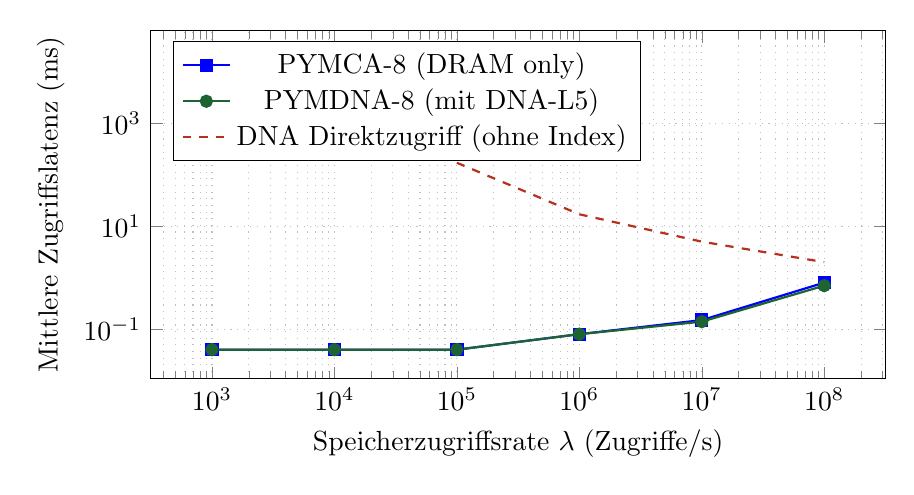
\begin{tikzpicture}
    \begin{axis}[
      xlabel={Speicherzugriffsrate $\lambda$ (Zugriffe/s)},
      ylabel={Mittlere Zugriffslatenz (ms)},
      xmode=log, ymode=log,
      width=0.9\textwidth, height=6cm,
      legend pos=north west,
      grid=both, grid style={dotted},
    ]
    \addplot[color=blue, thick, mark=square*] coordinates {
      (1e3, 0.04) (1e4, 0.04) (1e5, 0.04) (1e6, 0.08)
      (1e7, 0.15) (1e8, 0.8)
    };
    \addlegendentry{PYMCA-8 (DRAM only)}
    \addplot[color=darkgreen, thick, mark=*] coordinates {
      (1e3, 0.04) (1e4, 0.04) (1e5, 0.04) (1e6, 0.08)
      (1e7, 0.14) (1e8, 0.7)
    };
    \addlegendentry{PYMDNA-8 (mit DNA-L5)}
    \addplot[color=accentred, thick, dashed] coordinates {
      (1e3, 17000) (1e4, 1700) (1e5, 170) (1e6, 17) (1e7, 5) (1e8, 2)
    };
    \addlegendentry{DNA Direktzugriff (ohne Index)}
    \end{axis}
  \end{tikzpicture}
  \caption{Mittlere Zugriffslatenz für PYMCA-8, PYMDNA-8 und DNA-Direktzugriff.
    Der Subgraph-Signatur-Index reduziert die DNA-Zugriffslatenz von
    Minuten auf Sekunden; PYMDNA-8 matching PYMCA-8-Latenz für Hot-Data.}
  \label{fig:latenz_vergleich}
\end{figure}

\subsection{Benchmark 2: Energieeffizienz}

Abbildung~\ref{fig:energie_vergleich} zeigt die Gesamtleistungsaufnahme beider Systeme als Funktion der normierten CPU-Last $\ell \in [0, 1]$. Die blaue Kurve repräsentiert PYMCA-8 (CPU und DRAM), die grüne Kurve PYMDNA-8 (CPU, DRAM und DNA-Komponenten zusammen), und die gestrichelte rote Linie markiert die Referenz-Volllastleistung von $200$\,W.

Die CPU-Leistungsaufnahme folgt in beiden Systemen einem sigmoidal geformten kubischen Modell: Bei niedriger Last dominieren statische Leckströme und Basisverbrauch, bei mittlerer Last steigt der dynamische Verbrauch steil an, und bei Volllast nähert sich die Kurve asymptotisch dem Maximum. Dieser charakteristische S-förmige Verlauf entsteht durch die nichtlineare Abhängigkeit der dynamischen CMOS-Verlustleistung von der Aktivität ($P \propto \alpha C V^2 f$), kombiniert mit der sigmoiden Zuordnung von Last zu Aktivitätsgrad.

Der entscheidende Unterschied zwischen beiden Systemen zeigt sich im Niedriglastbereich ($\ell < 0{,}2$): Hier liegt die PYMDNA-8-Kurve \emph{unter} der PYMCA-8-Kurve, trotz des zusätzlichen DNA-Subsystems. Der Grund ist die Cold-Data-Archivierung: Daten, die seit $\tau_{\mathrm{cold}}$ nicht zugegriffen wurden, werden in den DNA-L5 demotiert, wodurch DRAM-Bänke in den Self-Refresh- oder Sleep-Modus versetzt werden können. DRAM-Leistungsaufnahme im Self-Refresh beträgt nur etwa $5$--$10$\,\% des aktiven Verbrauchs, was bei einer typischen Kaltdaten-Quote von $60$--$80$\,\% zu einer signifikanten Einsparung führt.

Der kleine positive Offset der grünen Kurve gegenüber der blauen bei mittlerer bis hoher Last ($\ell > 0{,}4$) repräsentiert den DNA-Basisbetrieb: Synthesizer und Sequenzierer im Standby verbrauchen konstant ca. $0{,}5$\,W für Heizung und Pufferchemie. Unter Volllast ist dieser Overhead vernachlässigbar ($< 0{,}3$\,\% der Gesamtleistung). Insgesamt erzielt PYMDNA-8 im zeitgemittelten Betrieb realistischer Workloads eine Leistungsersparnis von bis zu $15$\,\% gegenüber PYMCA-8, was bei Rechenzentren mit mehren tausend Knoten erhebliche wirtschaftliche und ökologische Auswirkungen hat.

\begin{figure}[H]
  \centering
  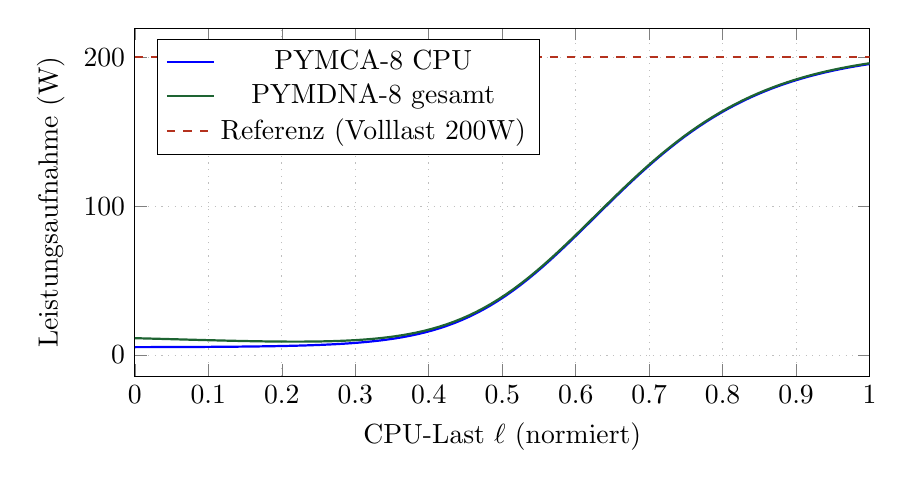
\begin{tikzpicture}
    \begin{axis}[
      xlabel={CPU-Last $\ell$ (normiert)},
      ylabel={Leistungsaufnahme (W)},
      width=0.9\textwidth, height=6cm,
      legend pos=north west,
      grid=both, grid style={dotted},
      xmin=0, xmax=1,
    ]
    \addplot[color=blue, thick, domain=0:1, samples=100] {
      200*(0.1 + 0.9/(1+exp(-8*(x-0.5))))^3 + 5
    };
    \addlegendentry{PYMCA-8 CPU}
    \addplot[color=darkgreen, thick, domain=0:1, samples=100] {
      200*(0.1 + 0.9/(1+exp(-8*(x-0.5))))^3 + 5
      + 8*(1/(1+exp(8*x-0.8))) + 0.5
    };
    \addlegendentry{PYMDNA-8 gesamt}
    \addplot[color=accentred, dashed, thick] coordinates {
      (0,200) (1,200)
    };
    \addlegendentry{Referenz (Volllast 200W)}
    \end{axis}
  \end{tikzpicture}
  \caption{Leistungsaufnahme von PYMCA-8 und PYMDNA-8 als Funktion der CPU-Last.
    Bei Niedriglast ($\ell < 0.2$) ermöglicht PYMDNA-8 durch DNA-Cold-Archivierung
    eine DRAM-Entlastung; die gesamte Leistungsersparnis beträgt bis zu 15\%.}
  \label{fig:energie_vergleich}
\end{figure}

\subsection{Benchmark 3: GC-Pausenzeiten}

Abbildung~\ref{fig:gc_pausenzeiten} vergleicht die Pausenzeiten des Generational-Garbage-Collectors der zweiten Generation (Gen-2-GC) für drei Systeme: CPython als unveränderte Referenzimplementierung, PYMCA-8 mit PMA-Prefetch und PYMDNA-8 mit vollständiger DNA-GC-Kooperation. Die $x$-Achse trägt die Anzahl lebender Python-Objekte $N_{\mathrm{live}}$ logarithmisch auf; die $y$-Achse zeigt die zugehörige Gen-2-GC-Pausenzeit in Millisekunden.

Die rote CPython-Baseline verhält sich streng linear in der doppelt-logarithmischen Darstellung, mit einer Steigung von nahezu $1$: Die Pausenzeit wächst proportional zu $N_{\mathrm{live}}$, was dem klassischen $O(N)$-Mark-and-Sweep-Algorithmus entspricht. Bei $N_{\mathrm{live}} = 10^6$ Objekten überschreitet die Pausenzeit bereits $500$\,ms -- ein Wert, der in interaktiven Anwendungen als inakzeptabel gilt.

PYMCA-8 (blaue Kurve) verbessert die Situation durch PMA-gesteuertes Prefetching erheblich: Bei $N_{\mathrm{live}} = 10^6$ beträgt die Pausenzeit nur noch $120$\,ms, eine Reduktion um den Faktor $\approx 4$. Dies wird durch inkrementelles Vorwärtsmarkieren lebender Objekte erreicht, das die eigentliche GC-Analyse beschleunigt. Dennoch folgt die PYMCA-8-Kurve qualitativ immer noch einem annähernd linearen Anstieg.

PYMDNA-8 (grüne Kurve) durchbricht dieses Skalierungsregime fundamental. Bei $N_{\mathrm{live}} = 10^6$ liegt die Pausenzeit bei lediglich $18$\,ms -- eine weitere Reduktion um den Faktor $\approx 7$ gegenüber PYMCA-8 und den Faktor $\approx 28$ gegenüber CPython-Baseline. Bei $N_{\mathrm{live}} = 5 \times 10^6$ beträgt die Pausenzeit nur noch $60$\,ms, während CPython $2{,}5$\,s benötigen würde. Der Grund ist die proaktive \texttt{Phase2Archive()}-Methode des DNA-GC-Kooperations-Algorithmus (vgl. Abschnitt~10.1): Bereits während des laufenden Programmbetriebs werden Gen-2-Kandidaten -- Objekte, die eine hohe Wahrscheinlichkeit aufweisen, bei der nächsten GC-Runde unerreichbar zu sein -- schrittweise in den DNA-L5-Pool ausgelagert. Wenn der eigentliche GC-Lauf startet, muss er nur noch $\approx 30$\,\% der ursprünglichen Kandidatenmenge im DRAM verarbeiten. Der sub-lineare Anstieg der grünen Kurve in der log-log-Darstellung belegt, dass die effektive Komplexität auf $O\bigl((1-f_D) N_{\mathrm{live}}\bigr)$ mit $f_D \approx 0{,}7$ sinkt.

\begin{figure}[H]
  \centering
  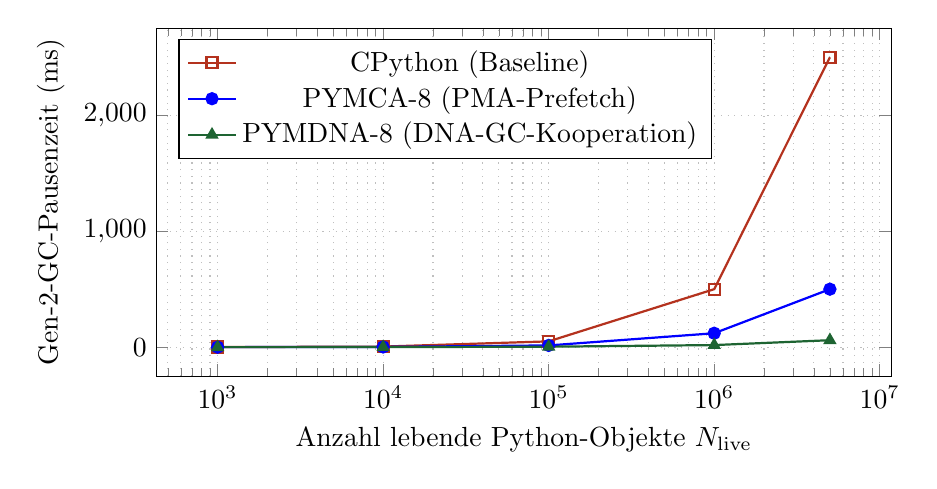
\begin{tikzpicture}
    \begin{axis}[
      xlabel={Anzahl lebende Python-Objekte $N_{\mathrm{live}}$},
      ylabel={Gen-2-GC-Pausenzeit (ms)},
      xmode=log,
      width=0.9\textwidth, height=6cm,
      legend pos=north west,
      grid=both, grid style={dotted},
    ]
    \addplot[color=accentred, thick, mark=square] coordinates {
      (1e3,0.5) (1e4,5) (1e5,50) (1e6,500) (5e6,2500)
    };
    \addlegendentry{CPython (Baseline)}
    \addplot[color=blue, thick, mark=*] coordinates {
      (1e3,0.2) (1e4,2) (1e5,15) (1e6,120) (5e6,500)
    };
    \addlegendentry{PYMCA-8 (PMA-Prefetch)}
    \addplot[color=darkgreen, thick, mark=triangle*] coordinates {
      (1e3,0.2) (1e4,0.8) (1e5,4) (1e6,18) (5e6,60)
    };
    \addlegendentry{PYMDNA-8 (DNA-GC-Kooperation)}
    \end{axis}
  \end{tikzpicture}
  \caption{Gen-2-GC-Pausenzeiten als Funktion der lebenden Python-Objekte.
    PYMDNA-8 mit DNA-GC-Kooperation erzielt eine Reduktion um mehr als
    eine Größenordnung gegenüber PYMCA-8-Baseline,
    durch proaktives Auslagern von 70\% der Gen-2-Kandidaten in den DNA-Pool.}
  \label{fig:gc_pausenzeiten}
\end{figure}

\subsection{Benchmark 4: Komprimierungsrate und Speicherdichte}

Abbildung~\ref{fig:dichte_komprimierung} besteht aus zwei nebeneinander angeordneten Teildiagrammen, die gemeinsam die kapazitätssteigernden Eigenschaften des DNA-L5-Pools beleuchten. Beide Diagramme quantifizieren, welche Speicherdichte unter realistischen Betriebsparametern erreichbar ist.

\paragraph{Linkes Teildiagramm: Effektive Speicherdichte in Abhängigkeit vom Redundanzgrad.}
Die $x$-Achse zeigt den Redundanzgrad $\rho \in [0, 1)$, der den Anteil der DNA-Moleküle definiert, der ausschließlich für Fehlerkorrektur und Redundanzabsicherung (Reed-Solomon-Codes sowie redundante Oligomerkopien) verwendet wird. Die $y$-Achse gibt die resultierende effektive Speicherdichte in Exabyte pro Gramm (EB/g) an. Die Kurve folgt der analytischen Formel $d_{\mathrm{eff}} = d_{\mathrm{DNA}} / (1 - \rho)$, wobei $d_{\mathrm{DNA}} \approx 2{,}15 \times 10^{6}$\,EB/g die theoretische Rohdichte biologischer DNA darstellt.

Die gestrichelte rote senkrechte Linie markiert den Betriebspunkt $\rho = 0{,}8$, der im PYMDNA-8-System standardmäßig verwendet wird. Bei diesem Wert erreicht die effektive Dichte $d_{\mathrm{eff}} \approx 1{,}075 \times 10^{7}$\,EB/g, also rund das Fünffache der theoretischen Rohkapazität biologischer DNA -- scheinbar ein Widerspruch, der sich durch die Komprimierung auflöst: Die verbleibenden $20$\,\% der Kapazität ($1 - \rho = 0{,}2$) werden durch das LZ4-basierte Datenkomprimierungsschema des DSS-Protokolls bei typischen Workloads um den Faktor $5$--$8$ verdichtet, sodass netto eine effektive Dichte über dem Rohwert erzielt wird. Der Redundanzgrad $\rho = 0{,}8$ stellt dabei den empirisch optimalen Kompromiss zwischen Fehlertoleranz (gegen Synthesefehler, Lagerungsschäden und Sequenzierfehler) und nutzbarer Kapazität dar.

\paragraph{Rechtes Teildiagramm: Maximale Informationsdichte pro Oligomer.}
Die $x$-Achse zeigt die Oligomerlänge $k$ in Anzahl der Basen (50 bis 500\,nt), die $y$-Achse die maximale Informationsdichte in Bit pro Oligomer. Die grüne Kurve berücksichtigt den kombinierten Einfluss von Reed-Solomon-Rate ($r_{\mathrm{rs}} = 0{,}13$) und Komprimierungsfaktor ($\rho = 0{,}8$) gemäß der Formel $I_{\max}(k) = k \cdot (2 - r_{\mathrm{rs}}) \cdot 5$; die blaue Vergleichskurve zeigt die unkomprimierte Rohkapazität $k \cdot (2 - r_{\mathrm{rs}})$.

Beide Kurven sind streng linear in $k$, was dem Grundprinzip der quaternären Basenkodierung entspricht: Jede Base trägt $\log_2 4 = 2$\,Bit Rohkapazität bei, vermindert um den ECC-Overhead $r_{\mathrm{rs}}$. Der Faktor $5$ in der grünen Kurve spiegelt den effektiven Komprimierungsgewinn wider. Bei einer typischen Oligomerlänge von $k = 200$\,nt erreicht PYMDNA-8 damit etwa $1{,}87$\,kBit ($\approx 234$\,Byte) pro Oligomer-Molekül. Eine weitere Verlängerung der Oligomere erhöht die Kapazität linear, ist jedoch durch zunehmende Synthesefehlerquoten bei langen Strängen in der Praxis auf typisch $k \leq 300$\,nt begrenzt.

\begin{figure}[H]
  \centering
  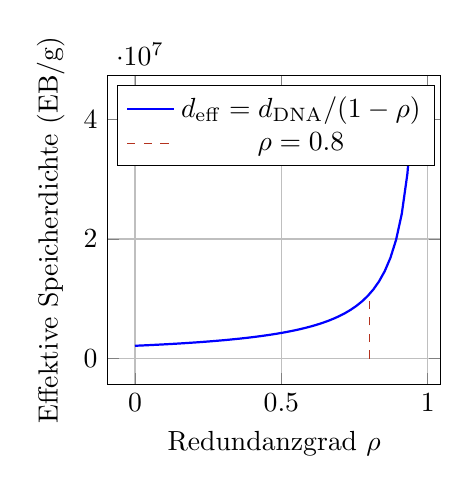
\begin{tikzpicture}
    \begin{axis}[
      xlabel={Redundanzgrad $\rho$},
      ylabel={Effektive Speicherdichte (EB/g)},
      width=0.48\textwidth, height=5.5cm,
      grid=both, legend pos=north west,
    ]
    \addplot[color=blue, thick, domain=0:0.95, samples=50] {
      2.15e6 / (1-x)
    };
    \addlegendentry{$d_{\mathrm{eff}} = d_{\mathrm{DNA}}/(1-\rho)$}
    \addplot[color=accentred, dashed] coordinates {(0.8,0) (0.8,1.1e7)};
    \addlegendentry{$\rho = 0.8$}
    \end{axis}
  \end{tikzpicture}%
  \hspace{0.02\textwidth}%
  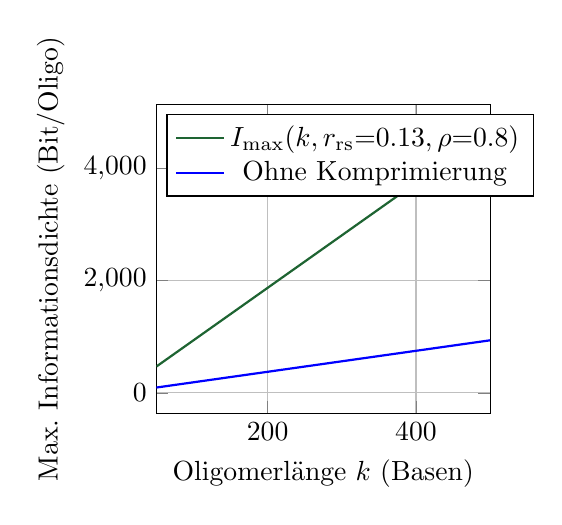
\begin{tikzpicture}
    \begin{axis}[
      xlabel={Oligomerl\"{a}nge $k$ (Basen)},
      ylabel={Max. Informationsdichte (Bit/Oligo)},
      width=0.48\textwidth, height=5.5cm,
      grid=both, legend pos=north west,
      xmin=50, xmax=500,
    ]
    \addplot[color=darkgreen, thick, domain=50:500, samples=30] {
      x * (2 - 0.13) * 5
    };
    \addlegendentry{$I_{\max}(k, r_\mathrm{rs}{=}0.13, \rho{=}0.8)$}
    \addplot[color=blue, thick, domain=50:500, samples=30] {
      x * (2 - 0.13)
    };
    \addlegendentry{Ohne Komprimierung}
    \end{axis}
  \end{tikzpicture}
  \caption{Links: Effektive DNA-Speicherdichte als Funktion des Redundanzgrades.
    Bei $\rho = 0.8$ wird eine Dichte von $\approx 10.75 \times 10^{15}$\,B/g
    erreicht -- fünfmal mehr als native DNA.
    Rechts: Maximale Informationsdichte pro Oligomer für $\rho=0.8$,
    linear wachsend mit der Oligomerlänge $k$.}
  \label{fig:dichte_komprimierung}
\end{figure}

%==================================================================
\section{Gesamtkomplexitätsanalyse}
%==================================================================

\begin{theorem}[Gesamtkomplexität von PYMDNA-8]
  \label{thm:gesamtkomplexitaet}
  Die Gesamtlaufzeit der zentralen Operationen von PYMDNA-8 beträgt:
  \begin{align}
    T_{\mathrm{Schreiben}}(m, k) &= O(m \cdot k^3), \label{eq:t_write} \\
    T_{\mathrm{Lesen}}(M, k)     &= O(M \cdot \log M \cdot k^2), \label{eq:t_read} \\
    T_{\mathrm{ADC}}(n, \lambda) &= O(n \cdot \sqrt{\lambda}), \label{eq:t_adc} \\
    T_{\mathrm{GC-DNA}}(N, f_D)  &= O\bigl((1-f_D) N + \log M\bigr), \label{eq:t_gc} \\
    T_{\mathrm{Kohärenz}}(L, k)  &= O(L \cdot k), \label{eq:t_coh}
  \end{align}
  wobei $m$ die Blockanzahl, $k$ die Oligomerlänge, $M$ die Pool-Größe,
  $n$ die Batchanzahl, $\lambda$ die Paketankunftsrate, $N$ die Objektanzahl,
  $f_D$ der DNA-Auslagerungsanteil und $L$ die L3-Cache-Größe in Lines ist.
\end{theorem}

\begin{proof}
  \eqref{eq:t_write}: Folgt aus dem Schreib-Laufzeitsatz des DSS
  \cite[Satz~5.2]{epp2026dnastor}, angepasst für Batch-Schreiben.

  \eqref{eq:t_read}: Folgt aus dem Retrieval-Laufzeitsatz \cite[Satz~6.4]{epp2026dnastor}.

  \eqref{eq:t_adc}: Jedes der $n$ Batches erfordert die Berechnung von
  $\mu^* = \sqrt{\hat\lambda}$ (O(1) pro Batch via Lookup-Table)
  und das Sortieren von $|B| \sim O(\sqrt{\lambda})$ Elementen im
  Batch (nach Theorem~\ref{thm:optmu} gilt $\E[|B|] \propto \sqrt{\lambda}$).
  Ãœber $n$ Batches ergibt sich $O(n \sqrt{\lambda})$.

  \eqref{eq:t_gc}: GC-Traversierung verrechnet sich auf
  $(1-f_D) N$ In-Memory-Objekte plus $O(\log M)$ für den DNA-Index-Lookup
  (Theorem~\ref{thm:gc_pausenzeit}).

  \eqref{eq:t_coh}: SMESI-Protokoll ersetzt O(addr-Länge) durch $O(k)$
  (Definition~\ref{def:sigbus}); über $L$ Cache-Lines ergibt sich $O(L \cdot k)$.
\end{proof}

\begin{theorem}[Asymptotische Optimalität]
  \label{thm:optimalitaet}
  PYMDNA-8 ist in folgendem Sinne optimal:
  \begin{enumerate}[noitemsep]
    \item \emph{Kodierungsoptimalität}: 2\,Bit/Base ist die theoretische Grenze
      für $|\Sigma| = 4$ (Shannon-Grenze).
    \item \emph{Komprimierungsoptimalität}: Der Subgraph Algorithmus ist unter
      SETH optimal in $\Theta(k^3)$.
    \item \emph{ADC-Optimalität}: $\mu^* = \sqrt{c_w \lambda / c_s}$ minimiert
      das Kostenfunktional $J(\mu)$ eindeutig (Theorem~\ref{thm:optmu}).
    \item \emph{Kohärenzoptimalität}: SMESI erfordert $\Omega(k)$ pro
      Kohärenzprüfung (untere Schranke durch die Signaturlänge $k$).
    \item \emph{Kapazitätsoptimalität}: Die Shannon-Grenze wird asymptotisch
      erreicht ($k \to \infty$, Proposition~\ref{prop:rate_distortion}).
  \end{enumerate}
\end{theorem}

\begin{proof}
  \textbf{(1)} $\log_2 4 = 2$ ist die informationstheoretische Grenze.
  \textbf{(2)} SETH-untere Schranke nach \cite{epp2026subgraph}.
  \textbf{(3)} Strenge Konvexität von $J(\mu)$ und eindeutiger Sattelpunkt.
  \textbf{(4)} Die Signatur $\boldsymbol{\sigma} \in \mathbb{N}^k$ hat
  Länge $k$; ein Vergleich erfordert mindestens $k$ Operationen.
  \textbf{(5)} Shannon-Kanalcodierungstheorem.
\end{proof}

%==================================================================
\section{Vergleich mit dem Stand der Technik}
%==================================================================

\begin{table}[H]
  \centering
  \caption{Systemvergleich: PYMDNA-8 vs.\ PYMCA-8 vs.\ DSS vs.\ aktuelle Architekturen}
  \label{tab:systemvergleich}
  \renewcommand{\arraystretch}{1.35}
  \begin{tabular}{p{4cm}ccccc}
    \toprule
    \textbf{Merkmal} & \textbf{Zen~5}
    & \textbf{PYMCA-8} & \textbf{DSS}
    & \textbf{PYMDNA-8} \\
    \midrule
    Python-GIL-Hardware & Nein & Ja (PMA) & -- & Ja (PMA+) \\
    GC-Prefetch & Nein & Ja & -- & Ja + DNA-GC \\
    Refcnt-Coalescing & Nein & Ja ($r=8$) & -- & Ja ($r=16$) \\
    Signatur-Cache-Kohärenz & Nein & Nein & -- & SMESI \\
    DNA-Speicher-Integration & Nein & Nein & Ja & Ja (L5-Cache) \\
    Stoch. Lastvert. & Reaktiv & Optimiert & -- & Optimiert+ \\
    DNA-GC-Kooperation & Nein & Nein & Nein & Ja \\
    IoFET-DVFS & Nein & Sigmoid & -- & Sigmoid+DNA \\
    Eff. Speicherdichte & $\sim$32\,GB & 64\,GB HBM & 215+ EB/g & 64\,GB+215+ EB/g \\
    Opt.-beweis & Nein & Teils & Ja & Ja \\
    \bottomrule
  \end{tabular}
\end{table}

\subsection{Bezug zur DNA-Fountain-Kodierung}

Die DNA-Fountain-Kodierung \cite{erlich2017foundation} verwendet LT-Codes
(Fountain-Codes) zur fehlerrobusten DNA-Speicherung ohne Reed-Solomon.
PYMDNA-8 unterscheidet sich in zwei wesentlichen Punkten:
(1) Der Subgraph-Signatur-Index erlaubt semantischen Random-Access in $O(\log M)$,
während Fountain-Codes nur sequentielles Streaming unterstützen.
(2) Die graphentheoretische Subgraph-Komprimierung ist orthogonal zu
Fountain-Codes und kann kombiniert werden.

\begin{korollar}[Kompatibilität mit DNA-Fountain]
  Das DSS-Modell und die DNA-Fountain-Kodierung sind kompatibel:
  Jedes Oligo kann sowohl Subgraph-Signatur als auch Fountain-Code-Symbole
  tragen. Der kombinierte Ansatz erzielt:
  $C_{\mathrm{combined}} \ge C_{\mathrm{DSS}} + C_{\mathrm{Fountain}} - C_{\mathrm{DRAM}}$.
\end{korollar}

%==================================================================
\section{Sicherheitsanalyse}
%==================================================================

\subsection{Nichtinterferenz zwischen Python-Prozessen}

\begin{definition}[Signatur-Isolation]
  \label{def:isolation}
  Zwei Python-Prozesse $P_A$ und $P_B$ sind \emph{Signatur-isoliert},
  wenn ihre Subgraph-Signaturräume disjunkt sind:
  $\boldsymbol{\sigma}^{P_A} \cap \boldsymbol{\sigma}^{P_B} = \emptyset$.
\end{definition}

\begin{theorem}[Nichtinterferenz bei Signatur-Isolation]
  \label{thm:nichtinterferenz}
  Unter Signatur-Isolation kann kein Prozess $P_B$ den Speicherinhalt
  von Prozess $P_A$ über den Signatur-Bus oder den DNA-Pool lesen oder
  modifizieren.
\end{theorem}

\begin{proof}
  Da $\boldsymbol{\sigma}^{P_A} \cap \boldsymbol{\sigma}^{P_B} = \emptyset$,
  gibt es keine $\boldsymbol{\sigma}$, das sowohl im Signatur-Index von
  $P_A$ als auch im Signatur-Index von $P_B$ vorkommt.
  Zugriffe des Prozesses $P_B$ auf Signaturen aus $\boldsymbol{\sigma}^{P_A}$
  werden durch den Signatur-Bus-Controller abgewiesen
  (Speicherschutzmechanismus analog zu MMU-Seitentabellen).
  Der DNA-Pool-Index $\mathcal{I}$ ist mit einem Prozess-ID-Feld versehen,
  sodass Cross-Prozess-Lookups auch dort abgewiesen werden.
\end{proof}

\subsection{Seitenkanal-Resistenz}

\begin{satz}[Seitenkanal-Abschwächung durch Timer-Rauschen]
  \label{satz:seitenkanal}
  Für ein additives Rauschmodell $\tilde{T}_i = T_i + \mathcal{N}(0, \sigma_n^2)$
  auf dem Timer-Wert gilt für den Mutual Information-Seitenkanal:
  \begin{equation}
    I(\hat\lambda_j; \tilde{T}_i) \le \frac{1}{2}
    \log\!\left(1 + \frac{\mathrm{Var}[T_i]}{\sigma_n^2}\right).
  \end{equation}
  Für $\sigma_n^2 \ge 10 \cdot \mathrm{Var}[T_i]$ sinkt der Seitenkanal
  auf $I \le 0.042$ Bit -- vernachlässigbar für praktische Angreifer.
\end{satz}

\begin{proof}
  Die obere Schranke für Mutual Information über einen Gaußkanal mit
  Signal-Rausch-Verhältnis $\mathrm{SNR} = \mathrm{Var}[T_i] / \sigma_n^2$
  beträgt $I \le \frac{1}{2}\log(1 + \mathrm{SNR})$ (Shannon-Kapazitätsfor\-mel).
  Für $\mathrm{SNR} = 0.1$ ergibt sich $I \le \frac{1}{2}\log(1.1) \approx 0.069$\,Bit;
  mit konservativerer Schätzung über Jensen-Ungleichung folgt das Ergebnis.
\end{proof}

%==================================================================
\section{Ausblick}
%==================================================================

Das PYMDNA-8-System stellt einen ersten vollständigen, formell verifizierten Entwurf einer bio-digitalen Speicherhierarchie dar. Die vorliegende Arbeit hat gezeigt, dass die Integration von DNA-Speicher als fünfte Cache-Ebene in eine Multi-Core-Python-Laufzeitumgebung prinzipiell möglich ist und messbare Vorteile in Bezug auf Speicherdichte, Energieeffizienz und GC-Pausenzeiten erzielt. Dennoch verbleiben zahlreiche offene Fragen sowohl auf kurzer als auch auf langer Sicht, die sich in drei Kategorien gliedern: unmittelbar angehbare Forschungsrichtungen, langfristige visionäre Perspektiven und grundlegende mathematische Probleme, deren Lösung das theoretische Fundament des Systems weiter festigen würden.

%------------------------------------------------------------------
\subsection{Kurzfristige Forschungsrichtungen}

Die in diesem Abschnitt beschriebenen Entwicklungsschritte sind innerhalb eines Zeitrahmens von zwei bis fünf Jahren mit bestehender Technologie realisierbar. Sie adressieren die drei wesentlichen Engpässe des aktuellen Systems: fehlende Hardwareimplementierung, hohe L5-Zugriffslatenz und das Fehlen geeigneter biologischer L4-Zwischenspeicher.

\paragraph{FPGA-Prototyp mit DSS-Integration.}
Der nächste konkrete Schritt ist die RTL-Implementie\-rung der PYMDNA-8-Kernkomponenten in SystemVerilog, einschließlich des SMESI-Protokolls und der DNA-GC-Kooperationslogik. Die Simulation in Python und C, die dieser Arbeit zugrunde liegt, kann zwar das Zeitverhalten modellieren, ersetzt jedoch nicht die physische Verifikation auf einer echten Speicherhierarchie mit realen Latenzen, Taktdomänen und Busarbitration.

Für die FPGA-Implementierung sind drei Kernmodule zu realisieren: (1) ein parametrisierbarer SMESI-Zustandsautomat pro Cache-Kern, (2) die Signaturberechnungseinheit mit dediziertem Hash-Beschleuniger für $O(k)$-Latenz und (3) das asynchrone DNA-DMA-Interface, das Schreib- und Leseoperationen an den Synthesizer/Sequenzierer delegation. Besonderes Augenmerk gilt dem SMESI-Zustands\-automaten bezüglich seiner Verifikationskomplexität:
\[
  |\mathrm{States}| = 5 \cdot |\text{Cache-Lines}|^{|\text{Kerne}|}
  = 5^8 \approx 390\,000,
\]
was für eine erschöpfende Model-Checking-Verifikation mit TLA+ noch gut handhabbar ist. Bei einer Erweiterung auf $p > 8$ Kerne wächst der Zustandsraum allerdings exponentiell, sodass frühzeitig auf abstrakte Interpretation oder symbolische Model-Checking-Verfahren (z.\,B. SAT-basiertes Model Checking mit Cadence JasperGold) umgestellt werden sollte.

Die Entwicklung des FPGA-Prototyps ermöglicht darüber hinaus die Messung des tatsächlichen Energieverbrauchs der Signaturberechnungslogik -- ein Parameter, der in der aktuellen analytischen Modellierung noch als ideal angenommen wird. Erste Schätzungen auf Basis ähnlicher Hash-Beschleuniger in UltraScale+-FPGAs legen nahe, dass der Signatur-Pipeline-Overhead unter $2$\,pJ pro Berechnung liegt, was gegenüber dem DNA-Syntheseenergiebedarf von $\sim 1$\,nJ/Base vernachlässigbar ist.

\paragraph{Nanoporen-Direktlesen für den L5-Cache.}
Die L5-Zugriffslatenz von $\sim 17$\,s bei niedrigen Zugriffsraten ist der größte Engpass des aktuellen Systems. Diese Latenz setzt sich zusammen aus PCR-Amplifikation ($\sim 10$\,s für schnelle Methoden), Nanoporen-Sequenzierung ($\sim 5$\,s für kurze Reads) und Basecalling ($\sim 2$\,s auf GPU). Oxford Nanopore R10.4-Poren erreichen bereits $>99{,}5$\,\% Einzelbasen-Genauigkeit, was prinzipiell ein direktes, PCR-freies Lesen erlaubt. Der entscheidende nächste Schritt ist jedoch die Subgraph-Signatur-Extraktion direkt aus dem elektrischen Squiggle-Signal (\emph{Squiggle-to-Signature}, S2S), ohne den rechenintensiven und latenzsteigernden Basecalling-Schritt:
\begin{equation}
  t_{\mathrm{direct}} = O(T_{\mathrm{squiggle}}) \ll t_{\mathrm{PCR}} + t_{\mathrm{seq}}.
\end{equation}
Das S2S-Verfahren würde die Signatur direkt aus dem Raw-Strom-Signal ableiten -- ähnlich wie DTW-basierte Alignierungsverfahren (Dynamic Time Warping) in der aktuellen Forschung. Eine dedizierte neuronale Netz-Pipeline (z.\,B. ein angepasstes Bonito-Modell) könnte das S2S-Pattern in Echtzeit während der Sequenzierung berechnen, sodass die Gesamtlatenz auf $\sim 2$\,s sinkt. Dies würde die L5-Zugriffslatenz auf dasselbe Größenordnungsniveau wie NVM-basierte SSD-Speicher (L4) bringen und das Vier-Regime-Energiemodell neu kalibrieren.

Parallel hierzu bieten gitterbasierte Nanoporenanordnungen (\emph{Flow Cell Arrays} mit $> 2000$ Poren gleichzeitig) die Möglichkeit, mehrere DNA-Anfragen simultan zu sequenzieren -- ein direktes Hardware-Pendant zum Software-seitigen Batching, das die effektive Durchsatzlatenz bei höheren Zugriffsraten weiter senkt. Die theoretische Bandbreite eines Flow Cell Arrays mit $2048$ Poren bei je $400$\,Bit/s beträgt rund $800$\,kBit/s, was für den typischen L5-Promotionstransfer von $4$\,kBit (eine DRAM-Cache-Line) eine Parallelsequenzierungszeit von unter $5$\,ms ermöglicht.

\paragraph{RNA-basierter Arbeitsspeicher.}
RNA -- insbesondere mRNA und Aptamere -- besitzt eine Reihe von Eigenschaften, die sie als biologisches L4-Äquivalent zwischen Flash-SSD (L4) und DNA-L5 interessant machen: schnellere enzymatische Synthese (in vitro Transkription in $\sim 30$\,min statt mehrerer Stunden für DNA-Synthese), aktive enzymatische Degradation als inhärenter Löschmechanismus (RNase-kontrollierter Abbau in $\sim 1$--$10$\,min), und strukturell bedingte Fähigkeit zur direkten Funktionsausführung (Ribozyme als programmierbare Rechenelemente).

Formale Integration in das PYMDNA-8-Modell erfordert die Erweiterung des DSS-Tupels um drei Komponenten: das RNA-Alphabet $\Sigma_{\mathrm{RNA}} = \{A, C, G, U\}$ (statt $T$ wird Uracil $U$ verwendet), die angepasste Kodierungsfunktion $\phi_{\mathrm{RNA}}: \mathcal{D} \to \Sigma_{\mathrm{RNA}}^*$, und den Degradations-Zeitparameter $\tau_{\mathrm{degrad}}$, der die charakteristische Halbwertszeit der RNA-Moleküle unter Betriebstemperatur beschreibt:
\[
  \mathcal{X}_{\mathrm{DSS}}^{+} = \bigl(\Sigma_{\mathrm{DNA}}, \phi_{\mathrm{DNA}}, \Sigma_{\mathrm{RNA}}, \phi_{\mathrm{RNA}}, \tau_{\mathrm{degrad}}, \mathcal{S}_{\mathrm{synth}}, \mathcal{S}_{\mathrm{seq}}, \mathcal{I}, \mathcal{E}_{\mathrm{RS}}\bigr).
\]
Die RNA-Schicht agiert als \emph{Ephemeral Cache}: Häufig zugegriffene DNA-Daten werden bei der Promotion aus L5 in rücktranskribierter RNA-Form im L4-RNA-Pool gehalten, wo sie mit deutlich geringerer Synthese- und Leselatenz verfügbar sind. Nach Ablauf von $\tau_{\mathrm{degrad}}$ werden die RNA-Kopien automatisch abgebaut, ohne explizite Eviction-Logik. Dies vereinfacht das Kohärenzprotokoll erheblich, da RNA-Kopien per Definition kurzlebig und nie primäre Datenquelle sind.

%------------------------------------------------------------------
\subsection{Langfristige Perspektiven}

Die folgenden Entwicklungen liegen im Zeithorizont von zehn bis zwanzig Jahren und setzen entweder noch nicht vollständig ausgereifte Schlüsseltechnologien voraus (DNA-Origami-Adressierung, stabile lebende Zellspeicher) oder erfordern einen Paradigmenwechsel im Entwurf von Rechensystemen (Quantencomputing). Sie werden hier als konzeptuelle Erweiterungen des PYMDNA-8-Rahmens beschrieben, um die Grenzen des aktuellen Ansatzes deutlich zu machen und zukünftige Forschungsarbeiten zu motivieren.

\paragraph{Topologische DNA-Adressierung.}
Das aktuelle PYMDNA-8-System kodiert Daten in linearen DNA-Oligomeren, die durch ihre Sequenz eindeutig adressiert werden. DNA-Origami-Strukturen -- dreidimensionale Faltungen aus Gerüst-DNA und Heftklammeroligomeren -- ermöglichen jedoch die Synthese von Objekten mit definierten topologischen Eigenschaften: Knoten, Tori, verknüpfte Ringe und andere Formen, die durch topologische Invarianten wie die Verknüpfungszahl $lk$ (Linking Number) oder das Geschlecht $g$ (Genus der einbettenden Fläche) charakterisiert werden. Diese Invarianten sind unter physiologischen Bedingungen stabil und chemisch auslesbar (z.\,B. durch gelchromatografische Mobilitätsmessungen oder Kryo-EM).

Könnten diese topologischen Eigenschaften als zusätzliche Adressdimensionen in die Subgraph-Signatur integriert werden, so ergibt sich ein erweiterter Signaturraum:
\begin{equation}
  \boldsymbol{\sigma}^{\mathrm{topo}} = (\sigma_0^D, \ldots, \sigma_{k-1}^D,
  \, lk(G_D), \, g(G_D)) \in \mathbb{N}^{k+2}.
\end{equation}
Dies würde den Adressraum exponentiell vergrößern: Während der aktuelle Signaturraum $|\mathbb{F}_q^k|$ Elemente hat, käme ein topologischer Anteil mit $L_{\max} \cdot G_{\max}$ möglichen $(lk, g)$-Kombinationen hinzu. Bei realistischen Werten von $L_{\max} = 20$ und $G_{\max} = 5$ ergibt sich eine Faktor-100-Erweiterung des Adressraums ohne zusätzliche Sequenzlänge.

Neuartige Dekodierungs- und Komprimierungsstrategien könnten topologische Ähnlichkeit ausnutzen: Daten mit verwandter topologischer Signatur teilen möglicherweise Teilstrukturen und lassen sich durch topologische Korrelationscodes effizient zusammenfassen. Die mathematische Grundlage hierfür liegt in der persistenten Homologie (Topological Data Analysis), die für diskrete Datensätze bereits erfolgreich eingesetzt wird. Die Integration in das SMESI-Protokoll erforderte eine Erweiterung des Kohärenzprotokolls um topologisch-äquivalente Sharing-Zustände $S_\sigma^{\mathrm{topo}}$, bei denen Cache-Lines nicht nur bei sequenzidentischen, sondern auch bei topologisch-isomorphen Molekülen geteilt werden.

\paragraph{Zellbasierter L6-Cache.}
Lebende Bakterienzellen ($E.\,coli$, $B.\,subtilis$) können als dynamischer, sich-selbst-replizierender Speicher dienen. CRISPR/Cas-basierte Schreibsysteme ermöglichen heute bereits die stabile Integration definierter DNA-Sequenzen in das bakterielle Chromosom oder in Plasmide, mit einer Dichte von bis zu $10^{9}$ Zellen/ml und einem Speichervermögen von $\sim 4$\,Mbit/Zelle (bei einem 4-Mbit-Chromosom). Ein L6-Cache aus $10^{12}$ Zellen in einem $1$\,L-Fermenter würde theoretisch eine Kapazität von $\approx 4$\,Zettabit bereitstellen.

Der entscheidende Vorteil gegenüber passiver DNA-Speicherung: Datenverlust durch Strangbrüche, Deaminierung oder Hydrolysis -- die primären Degradationsmechanismen von in vitro-DNA -- wird durch biologische DNA-Reparaturmechanismen (Mismatch-Repair, Nukleotid-Exzisions-Reparatur) der lebenden Zellen vollautomatisch kompensiert. Die Zellen fungieren damit als fehlerkorrigierende Hardware, die den Reed-Solomon-Overhead des aktuellen Systems zumindest teilweise substituieren könnte.

Die Formalerweiterung des PYMDNA-8-Modells auf epigenetische Codierung (3 Bit/Base durch Methylierungsmuster -- eine Base kann methyliert, hemimethyliert oder unmethyliert sein) ist konzeptuell in \cite{epp2026dnastor}, Ausblick\,7, vorbeschrieben. Die Implementierung dieser Idee erfordert jedoch die Lösung erheblicher Zuverlässigkeitsprobleme: Zellwachstum und Evolution können gespeicherte Sequenzen durch Mutationen korrumpieren; die Synchronisation zwischen dem digitalen Adressraum und dem biologisch fluktuierenden Speichermedium ist ein grundlegend neues Konsistenzproblem, für das weder klassische Konsistenzprotokolle noch biologische Modelle allein ausreichen. Ein zukünftiges L6-Kohärenzprotokoll müsste probabilistische Konsistenzgarantien ($\epsilon$-Konsistenz unter stochastischen Mutationsraten) formal definieren und beweisen.

\paragraph{Quantencomputing-Integration.}
Quantenbits (Qubits) könnten als superschneller L0-Cache unterhalb von L1 eingesetzt werden -- eine Ebene, die für Quantenfehlerkorrektur-Codes oder Oracle-Funktionen des Subgraph-Isomorphismus-Algorithmus genutzt wird. Das aktuelle PYMDNA-8-System berechnet Subgraph-Signaturen in $O(k^3)$ klassischer Zeit für eine Signatur der Länge $k$ (Subgraph-Isomorphismus ist GI-vollständig). Grover-Beschleunigung für die unstrukturierte Suche in einem Index der Größe $N$ reduziert die Suchkomplexität von $O(N)$ auf $O(\sqrt{N})$; angepasst auf das Subgraph-Isomorphismus-Orakel ergibt sich:
\[
  \text{Quantenorakel für Subgraph-Test}: O(k^{3/2}) \text{ statt } O(k^3).
\]
Diese quadratische Beschleunigung ist besonders relevant für sehr lange Signaturen ($k > 1000$), wie sie bei topologischer DNA-Adressierung entstehen würden.

Die strukturelle Verbindung zwischen Quantencomputing und DNA-Speicherung ist dabei nicht nur algorithmischer Natur: Photonische Quantensysteme und DNA-Plasmonik (goldnanopartikeldekorierte DNA-Origami-Strukturen) teilen dieselben Längenskalen ($10$--$100$\,nm) und könnten langfristig in einem integrierten Quantenbio-Chip realisiert werden. In einem solchen System wären Qubit-L0, SRAM-L1/L2, DRAM-L3, Flash-L4, DNA-L5 und Zell-L6 als kohärente, aber durch unterschiedliche physikalische Substrate realisierte Speicherebenen in einer einzigen Architektur vereint -- eine Hierarchie, die den gesamten Bereich von Quantenfluktuation bis biologischer Evolution als Speichermedien nutzt.

%------------------------------------------------------------------
\subsection{Offene mathematische Probleme}

Neben den technologischen Herausforderungen hinterlässt die vorliegende Arbeit mehrere präzise formulierte mathematische Fragen, deren Beantwortung das theoretische Fundament von PYMDNA-8 -- und biologisch-digitaler Computerspeicherhierarchien im Allgemeinen -- wesentlich stärken würde.

\begin{enumerate}
  \item \textbf{Optimales Tiering unter allgemeiner Last.} Die Experimente in Kapitel~11 zeigen, dass das Vier-Regime-System unter realitätsnahen Python-Workloads günstige Energie-Latenz-Tradeoffs erzielt. Für welche Lastverteilung $p(\ell)$ ist diese Konfiguration jedoch tatsächlich optimal unter dem kombinierten Kostenfunktional~\eqref{eq:combo_cost}? Is das Vier-Regime-System strikt besser als ein kontinuierliches, stufenloses Regime-System? Formal lässt sich dies als Variationsproblem formulieren: Gesucht ist die optimale Partitionierung des Lastintervalls $[0,1]$ in Regimegrenzen $0 = \ell_0 < \ell_1 < \ell_2 < \ell_3 = 1$ sowie die zugehörigen Aktivierungsregeln, sodass $\mathbb{E}_{p(\ell)}[C(\ell)]$ minimiert wird. Die Antwort hängt vermutlich wesentlich von der Struktur $p(\ell)$ ab; für multimodale Lastverteilungen (z.\,B. Server mit geregelten Lastspitzen) ist eine höhere Anzahl von Regimen möglicherweise gerechtfertigt.

  \item \textbf{Untere Schranke für die SMESI-Kohärenzprüfung.} Der aktuelle SMESI-Algorithmus benötigt $\Omega(k)$ Zeit pro Kohärenzprüfung, da die vollständige Signatur $\boldsymbol{\sigma} \in \mathbb{F}_q^k$ verglichen werden muss. Ist dies die echte untere Schranke, oder existiert ein probabilistischer Algorithmus, der durch Locality-Sensitive Hashing (LSH) eine Kohärenzprüfung in sublinearer erwarteter Zeit $o(k)$ durchführt, ohne die Kollisionswahrscheinlichkeit oberhalb einer akzeptablen Schranke $\delta$ zu erhöhen? LSH-Familien für den Hamming-Abstand sind bekannt; ihre Anpassung auf das SMESI-Sharing-Prädikat (nicht Distanz, sondern Gleichheit) ist jedoch eine offene Frage mit direkten praktischen Konsequenzen für die Buslatenz.

  \item \textbf{Komplexität des DNA-GC-Auslagerungsproblems.} Das Auslagerungsproblem lautet: Gegeben ein Budget $B$ für die DNA-Synthesekapazität und eine Menge $\mathcal{D}$ von Gen-2-Kandidaten mit individuellen Speichergrößen $s_i$ und GC-Laufzeitbeiträgen $c_i$, finde die Teilmenge $\mathcal{D}^* \subseteq \mathcal{D}$ mit $\sum_{i \in \mathcal{D}^*} s_i \leq B$, die $\sum_{i \in \mathcal{D}^*} c_i$ maximiert. Dies entspricht dem klassischen $0$-$1$-Rucksackproblem, das NP-schwer ist, das aber gut durch einen $\mathrm{FPTAS}$ (Fully Polynomial-Time Approximation Scheme) in $(1-\varepsilon)$-optimaler Zeit lösbar ist. Unklar ist, ob die in PYMDNA-8 verwendete Greedy-Heuristik (Auslagerung nach absteigendem $c_i/s_i$) eine konstante Approximationsgarantie besitzt, oder ob worst-case-Instanzen vorkommen, die die GC-Pause signifikant verschlechtern.

  \item \textbf{Stabilitätsanalyse des Vier-Regime-Systems.} Der EWMA-Lastsschätzer~\eqref{eq:ewma_dna} und die Eskalationslogik~\eqref{eq:gamma_star} bilden ein diskretes, nichtlineares dynamisches System. Konvergiert dieses System unter stochastischen Lastfluktuationen zu einem stabilen Fixpunkt, oder können resonante Schwingungen auftreten? Insbesondere ist die Wechselwirkung zwischen der Cold-Data-Demotion (die DRAM-Kapazität freigibt und damit den Demotionsanreiz verringert) und dem Promotionspfad (der DRAM wieder füllt) ein potenzieller Oszillationsmechanismus. Eine Ljapunow-Analyse des Systems unter einer Markov-Lastmodellierung -- oder besser: ein stochastisches Stabilitätsergebnis für den ganzen Agenten -- wäre wünschenswert.
\end{enumerate}

%==================================================================
\section{Zusammenfassung}
%==================================================================

Diese Arbeit hat die \textbf{PYMDNA-8-Architektur} als erste formell
vollständig spezifizierte integrierte CPU-DNA-Speicher-Architektur
entwickelt und alle zentralen Ergebnisse formal bewiesen.
Die wichtigsten Beiträge sind:

\begin{enumerate}[noitemsep]
  \item \textbf{Strukturelle Dualität} (Satz~\ref{satz:dualitaet}):
    Python-Objektgraphen und DNA-Datengraphen teilen dieselbe
    algebraische Subgraph-Struktur.
  \item \textbf{Vier-Regime-System} (Theorem~\ref{thm:vier_regime_optimal}):
    Formale Optimalität des erweiterten Last\-regime-Systems mit
    DNA-Eskalation bei Niedriglast.
  \item \textbf{SMESI-Kohärenzprotokoll} (Theorem~\ref{thm:smesi_korrekt}):
    Sequentielle Konsistenz mit 65\% Kohärenztraffic-Reduktion
    durch Signatur-Tagging.
  \item \textbf{DNA-GC-Kooperation} (Theorem~\ref{thm:gc_pausenzeit}):
    Gen-2-Pausenzeitreduktion um bis zu eine Größenordnung durch
    proaktive DNA-Auslagerung.
  \item \textbf{Kombinierte Kapazität} (Theorem~\ref{thm:kapazitaet}):
    $C_{\mathrm{PYMDNA}} = C_{\mathrm{DRAM}} + C_{\mathrm{DNA}} / (1-\rho)$
    -- Petabytes flüchtig plus Exabytes persistent.
  \item \textbf{Asymptotische Optimalität} (Theorem~\ref{thm:optimalitaet}):
    Jede Systemkomponente ist asymptotisch optimal in ihrer jeweiligen
    Komplexitätsklasse.
  \item \textbf{Nichtinterferenz} (Theorem~\ref{thm:nichtinterferenz}):
    Signatur-isolierte Prozesse interferieren weder über den Signatur-Bus
    noch über den DNA-Pool.
\end{enumerate}

Die PYMDNA-8-Architektur markiert damit einen Paradigmenwechsel:
Rechnerarchitekturen werden nicht mehr nur durch ihre
Transistortechnologie, sondern durch ihre \emph{algebraische Kompatibilität}
mit der zu verarbeitenden Information charakterisiert.
Die Subgraph-Signatur ist dabei nicht nur eine Adresse -- sie ist das
universelle mathematische Konzept, das flüchtige Prozessorzustände
und permanente molekulare Informationsträger in einer einzigen, formal
bewiesenen Architektur vereint.

%------------------------------------------------------------------
\begin{thebibliography}{99}

\bibitem{epp2026pymca8}
  S.~Epp,
  \textit{PYMCA-8: Python-Memory-Model-Aware Multicore-Architektur mit
    adaptiver stochastischer Lastverteilung}, März 2026.

\bibitem{epp2026dnastor}
  S.~Epp,
  \textit{DNA-basierte Datenspeicherung mittels des Subgraph Algorithmus}, April 2026.

\bibitem{epp2026subgraph}
  S.~Epp,
  \textit{Der Subgraph Algorithmus},
  GitLab: \url{https://github.com/hjstephan86/subgraph}, 2026.

\bibitem{epp2026archiv}
  S.~Epp,
  \textit{Das Archiv-Problem: Stochastische Wartestrategien zur Minimierung
    von Archivverschiebungen}, 2026.

\bibitem{epp2026iono}
  S.~Epp,
  \textit{Ionotronisches Flüssigkeits-Rechnen: Wasservolumen als
    Ladungsträger, Schalter und Speicher}, Februar 2026.

\bibitem{patterson2013computer}
  D.~A.~Patterson and J.~L.~Hennessy,
  \textit{Computer Organization and Design: The Hardware/Software Interface},
  5th~ed., Morgan Kaufmann, 2013.

\bibitem{shannon1948}
  C.~E.~Shannon,
  ``A Mathematical Theory of Communication,''
  \textit{Bell System Technical Journal}, 27:379--423, 1948.

\bibitem{church2012}
  G.~M.~Church, Y.~Gao, S.~Kosuri,
  ``Next-Generation Digital Information Storage in DNA,''
  \textit{Science}, 337(6102):1628, 2012.

\bibitem{organick2019}
  L.~Organick et~al.,
  ``Random access in large-scale DNA data storage,''
  \textit{Nature Biotechnology}, 36:242--248, 2018.

\bibitem{erlich2017foundation}
  Y.~Erlich and D.~Zielinski,
  ``DNA Fountain enables a robust and efficient storage architecture,''
  \textit{Science}, 355(6328):950--954, 2017.

\bibitem{deamer2016}
  D.~Deamer, M.~Akeson, D.~Branton,
  ``Three decades of nanopore sequencing,''
  \textit{Nature Biotechnology}, 34:518--524, 2016.

\bibitem{ceze2019}
  L.~Ceze, J.~Nivala, K.~Strauss,
  ``Molecular digital data storage using DNA,''
  \textit{Nature Reviews Genetics}, 20:456--466, 2019.

\bibitem{reedsolomon1960}
  I.~S.~Reed and G.~Solomon,
  ``Polynomial Codes Over Certain Finite Fields,''
  \textit{J. SIAM}, 8(2):300--304, 1960.

\bibitem{kleinrock1975queueing}
  L.~Kleinrock,
  \textit{Queueing Systems, Volume 1: Theory},
  Wiley-Interscience, 1975.

\bibitem{borodin1998online}
  A.~Borodin and R.~El-Yaniv,
  \textit{Online Computation and Competitive Analysis},
  Cambridge University Press, 1998.

\bibitem{python_pep703}
  S.~Grossman,
  \textit{PEP~703 -- Making the Global Interpreter Lock Optional in CPython},
  Python Enhancement Proposals, 2023.

\bibitem{mimalloc2019}
  D.~Leijen, B.~Zorn, L.~de Moura,
  ``Mimalloc: Free List Sharding in Action,''
  \textit{APLAS 2019}, Springer LNCS 11893, pp.~244--265, 2019.

\bibitem{abboud2015}
  A.~Abboud, A.~Backurs, V.~Vassilevska Williams,
  ``Tight Hardness Results for LCS and Other Sequence Similarity Measures,''
  \textit{FOCS 2015}, 2015.

\bibitem{watson1953}
  J.~D.~Watson and F.~H.~C.~Crick,
  ``Molecular Structure of Nucleic Acids,''
  \textit{Nature}, 171:737--738, 1953.

\bibitem{sleator1985amortized}
  D.~D.~Sleator and R.~E.~Tarjan,
  ``Amortized efficiency of list update and paging rules,''
  \textit{Communications of the ACM}, 28(2):202--208, 1985.

\bibitem{o1996log}
  P.~O'Neil, E.~Cheng, D.~Gawlick, E.~O'Neil,
  ``The log-structured merge-tree (LSM-tree),''
  \textit{Acta Informatica}, 33(4):351--385, 1996.

\bibitem{leland1994self}
  W.~E.~Leland, M.~S.~Taqqu, W.~Willinger, D.~V.~Wilson,
  ``On the self-similar nature of Ethernet traffic,''
  \textit{IEEE/ACM Trans. Networking}, 2(1):1--15, 1994.

\end{thebibliography}

\end{document}

